\documentclass{article}

\usepackage[utf8]{inputenc}
\usepackage[french]{babel}
\usepackage[T1]{fontenc}

\usepackage[a4paper, left=2cm, right=2cm, top=2.5cm, bottom=2.5cm]{geometry}
\usepackage{amssymb}
\usepackage{amsmath}
\usepackage{graphicx} % pour les images 
\usepackage{listings} % pour intégrer un code R
\usepackage{xcolor} % pour coloriser le code R intégré
\usepackage{comment}
\usepackage{float}
\usepackage{amsthm}
\usepackage{hyperref}



\theoremstyle{plain}
\newtheorem{definition}{Définition}[section]

\theoremstyle{definition}
\newtheorem{example}[definition]{Exemple}
\newtheorem{remark}[definition]{Remarque}

\theoremstyle{plain}
\newtheorem{theorem}[definition]{Théorème}
\newtheorem{lemma}[definition]{Lemme}
\newtheorem{proposition}[definition]{Proposition}
\newtheorem{property}{Propriété}
\newtheorem{exemplecustom}{Exemple}



\lstset{
	language=R,
	inputencoding=utf8, 
	extendedchars=true,       
	basicstyle=\ttfamily\footnotesize,
	keywordstyle=\color{blue},
	commentstyle=\color{green!50!black},
	stringstyle=\color{red},
	numbers=left,
	numberstyle=\tiny,
	stepnumber=1,
	breaklines=true,
	literate=%
	{é}{{\'e}}1
	{è}{{\`e}}1
	{ê}{{\^e}}1
	{à}{{\`a}}1
	{ù}{{\`u}}1
	{ç}{{\c{c}}}1
}

\title{\Huge \textbf{Étude des valeurs extrêmes univariées}}
\author{El Mazzouji Wahel, Mariac Damien, Condamy Fabian} 
\date{\today} 

\begin{document}

\maketitle 

\begin{center}
	\vspace{4cm} 
	
\includegraphics[width=0.4\textwidth]{./images/LogoSSD.png} 
\end{center}

\newpage
\tableofcontents 
\newpage
\section{Introduction}
Les événements extrêmes, comme les crues, les canicules ou les krachs financiers, sont rares mais peuvent avoir des conséquences majeures. Leur étude est devenue essentielle dans des domaines comme la climatologie, la finance ou l’assurance.

La théorie des valeurs extrêmes fournit un cadre statistique pour analyser ces phénomènes rares. Contrairement aux méthodes classiques, centrées sur la moyenne ou la variance, elle se concentre sur les plus grandes ou plus petites observations.

Alors que le théorème central limite traite des moyennes, la théorie des valeurs extrêmes s’intéresse au comportement du maximum d’un échantillon :
\[
M_n = \max\{X_1, X_2, \dots, X_n\}.
\]

Les travaux de Fréchet, Fisher, Tippett et Gnedenko ont montré que ce maximum, après normalisation, converge vers l’une des trois lois limites : Fréchet, Gumbel ou Weibull. Ces lois permettent de modéliser différentes formes de queues de distribution.

En se focalisant sur les extrêmes, la théorie des valeurs extrêmes offre des outils puissants pour anticiper la fréquence et l’intensité des événements rares.
\section{Comportement asymptotique de $M_n$}

\subsection{Caractérisation avec la fonction de répartition}

\noindent On commence par faire une remarque (\textit{Stochastic Modelling 1988}) sur la fonction de repartion de $M_n$ en utilisant le fait que les $X_i$ sont i.i.d.
En effet, si on note $F_{M_n}$ la fonction de repartition de $M_n$, et $F$ la fonction de repartition de $X_i$ on a :
\[
\forall t \in \mathbb{R} , \quad F_{M_n}(t) = \mathbb{P}(M_n \le t) = \mathbb{P}(X_1 \le t,...,X_n \le t)=\mathbb{P}(X_1 \le t)^n = F^n(t) 
\]
\\
On déduit de cette forme que pour $t<t^*$ où $t^*$ est la borne supérieure du support des $X_i$, on a $F(t)<1$, 
\[
\text{et donc} \; \; F^n(t) \xrightarrow[n\to +\infty]{} 0,
\]
et dans le cas ou t est supérieur ou égal à $t^*$,
\[
\text{, on a} \; \; F^n(t) \xrightarrow[n\to +\infty]{} 1.
\]
L'idée derrière la théorie des valeurs extremes est d'introduire deux suites ($b_n$) et ($a_n$) (avec $a_n > $  0 pour tout $n$) afin d'avoir une limite non dégénérée pour le maximum en posant $\frac{M_n - b_n}{a_n}$. 
\\
On sait que la fonction de répartition caractérise la loi, donc il nous suffit d'étudier la fonction $G$ définie pour tout $t$ dans le support des $X_i$ comme :

\[
\mathbb{P} \left( \frac{M_n - b_n}{a_n} \le t \right) \xrightarrow[n\to +\infty]{} G(t)
\]
\\
S'il existe de telle suites $a_n$ et $b_n$, on dit que $F$ est dans \textbf{le domaine d'attraction} de $G$.
\\
\\
Nous utilisons cette définition de la convergence en loi (\textit{Statistics of Extremes, Jan Beirlant 2004}) :
\\
\\
\begin{definition}
\textbf{(Convergence en loi)}:
Soit \( Y_n \) une variable aléatoire de fonction de répartition \( F_n \), et soit \( Y \) une variable aléatoire de fonction de répartition \( F \).  
Alors $Y_n \xrightarrow{\mathcal{L} } Y$ si et seulement si pour toute fonction $z$ réelle, bornée et continue :
\[
\mathbb{E}[z(Y_n)] \xrightarrow[n\to +\infty]{} \mathbb{E}[z(Y)].
\]
\end{definition}
\noindent Dans notre context, on décide de poser $Y_n = \frac{M_n -b_n}{a_n}$ et sont ésperance devient : 
\[
\mathbb{E} \left[ z \left( \frac{M_n -b_n}{a_n} \right) \right] = \int_{-\infty}^{\infty} z \left( \frac{x-b_n}{a_n} \right) \: n \:  F^{n-1} (x)dF(x)
\]
\\
\\
Afin de pouvoir identifier la loi limite, on voudrait ramener l'intégrale sous la forme :
\[
\int_{-\infty}^{\infty} z(u) \, dG(u)
\]
On va alors procéder par un changement de variable. Mais avant on introduit la fonction quantile qui va nous être utilise à ses fin. Elle est définie par :
\\
\[
Q(p) \;=\; F^{-1}(p)
\;=\;
\inf\bigl\{x\in\mathbb{R}\,\bigm|\,F(x)\ge p\bigr\},
\quad p\in[0,1].
\]

\noindent On pose alors le changement de variable issue de \textit{Statistics of Extremes, Jan Beirlant 2004}: 

\[
x = Q(1-\frac{1}{y}) = U(y) \; \; \; \; \; \; 
\]

\begin{equation}\label{eq:1.1}
    \text{et on obtient} \; \; \int_{-\infty}^{\infty} z\Bigl(\frac{x-b_n}{a_n}\Bigr) \, n \, F^{n-1}(x)\,dF(x)
    =\int_{0}^{n} z\Bigl(\frac{U\Bigl(\frac{n}{v}\Bigr)-b_n}{a_n}\Bigr)
    \Bigl(1-\frac{v}{n}\Bigr)^{n-1}dv.
\end{equation}
\\
\\
Or, on a $\lim_{n \to \infty} ( 1 - \frac{v}{n})^{n-1} = e^{-v}$ , et on a pour la borne de l'intégrale $\lim_{n \to \infty} \mathbf{1}_{[0;n]}(x) = \mathbb{R}_{+}$.
\\
\\
Ce changement de variable nous conduit à exprimer l’espérance sous une nouvelle forme, dans laquelle les suites $(a_n)$ et $(b_n)$ sont choisies de manière à assurer la convergence vers une intégrale limite de type $\int_{-\infty}^{\infty} z(u)\, dG(u)$.


\subsection{Le paramètre $b_n$}

\noindent En reprenant les hypothèses, on remarque que pour tout $t\in\mathbb R$,
\[
\mathbb{P}  \Bigl(\frac{M_n - b_n}{a_n} \le t\Bigr)
\;=\;
\mathbb{P} \bigl(M_n \le a_n\,t + b_n\bigr)
\;=\;
F^{n}\bigl(a_n\,t + b_n\bigr).
\]
Ce qui donne avec la convergence en loi :
\[
\frac{M_n - b_n}{a_n}\;\overset{\mathcal{L}}{\xrightarrow[n\to +\infty]{}}\;Y
\quad\Longleftrightarrow\quad
\mathbb{P} \bigl(M_n \le a_n\,t + b_n\bigr)
\;\xrightarrow[n\to +\infty]{} \; G(t),
\]
qui se traduit exactement par :
\[
F^{n} \bigl(a_n t + b_n\bigr)
\;\xrightarrow[n\to\infty]{}\;
G(t).
\]

\noindent En passant au logarithme, on obtient :

\[
n \: \ln (F(a_n t + b_n)) \xrightarrow[n\to +\infty]{} \ln (G(t))
\]
En faisant un développement limité du logarithme :
\[
n(1 - F(a_n t + b_n)) \xrightarrow[n\to +\infty]{} - \ln (G(t))
\]
\\
\\
Le cas particulier de cette convergence pour $t=0$ et en passant à l'opposé donne :
\[
n\bigl(F(b_n)-1\bigr)\;\xrightarrow[n\to\infty]{}\; \ln G(0)
\]
Comme on souhaite une limite non-dégénérée et non nulle, on impose :
\[
n\bigl[1 - F(b_n)\bigr] \;=\; 1.
\]
Il vient alors en composant par la fonction quantile :
\[
F(b_n)=1-\frac1n
\quad\Longleftrightarrow\quad
b_n \;=\; Q\!\Bigl(1-\tfrac1n\Bigr)
\;=\;U(n),
\]
 On obtient alors une forme explicite pour la suite $(b_n)$ qui est $U(n)$.

\subsection{Le paramètre $a_n$}
\noindent Une fois la suite $(b_n)$ fixée comme précédemment, nous devons maintenant déterminer la suite $(a_n)$. Il n'existe pas de forme explicite à celle-ci. L’objectif est alors de trouver des
 conditions suffisantes sur la fonction de répartition $F$ pour garantir l’existence d’une loi limite non dégénérée de $\frac{M_n - b_n}{a_n}$.
\\

\noindent En reprenant la convergence  $F^n(a_n t + b_n) \longrightarrow G(t)$, cela implique, en inversant \( G \) :
\[
a_n t + b_n = G^{-1}(F^n(a_n t + b_n)) \longrightarrow G^{-1}(G(t)) = t.
\]

\noindent En posant \( U(y) = Q\left(1 - \frac{1}{y}\right) \), on en déduit, pour de grandes valeurs de \( x \), que la convergence en loi est équivalente à la convergence des quantiles :
\[
\frac{U(xu) - U(x)}{a(x)} \longrightarrow h(u),
\]
où \( h(u) \) dépend du domaine d’attraction de \( F \). \\

\noindent Cette condition traduit, en quelque sorte, une régularité asymptotique de la queue de distribution.


\begin{remark}
	L'inversion de $G$ est bien définie via la fonction quantile que l'on a définie. On a posé $G^{-1}$ la fonction quantile associé à $G$.
\end{remark}

\vspace{0.3cm}
\noindent Il reste à étudier las limites possible, pour cela nous avons la proposition suivante (\textit{Statistics of Extremes, Jan Beirlant 2004}) :
\vspace{0.3cm}
\begin{proposition}[Limites possibles de la fonction $h$]
Les fonctions limites possibles sont données, pour une certaine constante $c > 0$, par :
\[
c \cdot h_\gamma(u) = c \int_1^u v^{-\gamma - 1} \, dv = \frac{c(u^\gamma - 1)}{\gamma}.
\tag{2}
\]

\noindent Nous interprétons la fonction limite dans le cas $\gamma = 0$ par passage à la limite :

\[
h_0(u) = \log(u).
\]
\end{proposition}

\noindent
\begin{remark}
	La constante $c$ ne peut pas être nulle, car cela conduirait à une limite dégénérée pour la variable normalisée $\frac{M_n - b_n}{a_n}$. En pratique, on peut toujours ramener le cas $c > 0$ au cas $c = 1$ en absorbant $c$ dans la définition de la fonction $a$.
\end{remark}

\vspace{0.5cm}

\begin{proof} 
Soient $u, v > 0$. Pour étudier la limite
\[
\lim_{x \to \infty} \frac{U(xu) - U(x)}{a(x)} = h(u),
\]
nous cherchons à établir une structure fonctionnelle sur la fonction limite $h(u)$. \\

\noindent Pour cela, nous considérons l’expression étendue :
\[
\frac{U(xuv) - U(x)}{a(x)},
\]
qui, par hypothèse, converge vers $h(uv)$ lorsque $x \to \infty$. Cette forme généralisée permet de relier $h(uv)$ à $h(u)$ et $h(v)$ en introduisant un point intermédiaire $xu$.

\noindent Nous décomposons alors l’expression :
\[
\frac{U(xuv) - U(x)}{a(x)} =
\frac{U(xuv) - U(xu)}{a(xu)} \cdot \frac{a(xu)}{a(x)} +
\frac{U(xu) - U(x)}{a(x)}.
\tag{3}
\]

\noindent Par hypothèse de convergence, on sait que :
\[
\lim_{x \to \infty} \frac{U(xu) - U(x)}{a(x)} = h(u),
\quad \text{et} \quad
\lim_{x \to \infty} \frac{U(xuv) - U(xu)}{a(xu)} = h(v).
\]

\noindent On suppose également que la fonction $a(x)$ satisfait la propriété de régularité suivante :
\[
\lim_{x \to \infty} \frac{a(xu)}{a(x)} = g(u),
\]
pour une certaine fonction positive $g(u)$. \\

\noindent En reportant ces limites dans l'équation (3), on obtient :
\[
\lim_{x \to \infty} \frac{U(xuv) - U(x)}{a(x)} = h(v) \cdot g(u) + h(u),
\]
ce qui donne :
\[
h(uv) = h(v) \cdot g(u) + h(u).
\tag{4}
\]

\noindent Cette relation impose une structure fonctionnelle entre $h$ et $g$. Pour que l'équation (4) soit cohérente pour tout $u, v > 0$, la fonction $g$ doit satisfaire l'équation fonctionnelle multiplicative :
\[
g(uv) = g(u) g(v),
\]
connue sous le nom d’équation de Cauchy multiplicative. \\

\noindent Les solutions mesurables et positives de cette équation sont les fonctions puissance, soit :
\[
g(u) = u^{\gamma} \quad \text{pour un certain } \gamma \in \mathbb{R}.
\]

\noindent On en déduit que $a(x)$ est une fonction à \textit{variation régulière} d’indice $\gamma$, ce qui signifie :
\[
\frac{a(xu)}{a(x)} \longrightarrow u^\gamma \quad \text{quand } x \to \infty.
\]

\noindent En remplaçant cette forme de $g(u)$ dans l’équation (4), on obtient :
\[
h(uv) = h(v) \cdot u^\gamma + h(u).
\]

\noindent Cette équation admet comme solution (admis) (à une constante multiplicative près) :
\[
h(u) = c \cdot \frac{u^\gamma - 1}{\gamma}, \quad \text{pour } \gamma \neq 0.
\]

\noindent Dans le cas limite $\gamma = 0$, par passage à la limite, on retrouve :
\[
h_0(u) = c \cdot \log u.
\]

\noindent On adopte la convention $h_0(u) = \log u$ en fixant $c = 1$, ce qui permet de résumer :
\[
h_\gamma(u) = \frac{u^\gamma - 1}{\gamma}, \quad \text{avec } h_0(u) = \log u.
\]

\end{proof}	
\subsection{Les lois limites}
\noindent En reprenant $(3)$ et en utilisant ce qui précède, on obtient :
\[
\lim_{x\to \infty} \frac{U(xuv) - U(x)}{a(x)} = u^{\gamma} h(v) + h(u)
\]
\[
\text{autrement dit :} \; \; h_{\gamma}(uv)= u^{\gamma} h_{\gamma}(v) + h_{\gamma}(u)
\]
En reprenant le résultat de la proposition 2.2 et ce qui précède  $(2)$, on obtient :
\[
h_\gamma\Bigl(\frac{1}{v}\Bigr)=\frac{(1/v)^\gamma-1}{\gamma}=\frac{v^{-\gamma}-1}{\gamma}
\]
Posons \(u=\frac{v^{-\gamma}-1}{\gamma}\). On résout alors pour \(v\) :
\[
v^{-\gamma}=1+\gamma u\quad\Longrightarrow\quad v=(1+\gamma u)^{-1/\gamma}
\]
Le changement de variable de \(v\) à \(u\) permet de réécrire l'intégrale limite sous la forme
\[
\int_{u\in S_\gamma} z(u)\,d\Bigl\{\exp\Bigl[-\left(1+\gamma u\right)^{-1/\gamma}]\Bigr\}
\]
ce qui conduit à identifier la loi limite par
\[
G_\gamma(u)=\exp\Bigl\{-\left(1+\gamma u\right)^{-1/\gamma}\Bigr\}
\]
Il reste alors à étudier la nature du support \(S_\gamma\), mais celui-ci dépend du signe de \(\gamma\).
\\
On fait alors une disjonction de cas sur la valeur de $\gamma$.
\\
\\
\textbf{\underline{Cas si \(\gamma>0 : \)}}
\\
\\
L'inversion montre que \(v\in [0,1]\) correspond à \(u>-\frac{1}{\gamma}\).
\\
\\
De plus, pour de grandes valeurs \(x\) on a :
\[
S_{\gamma} \approx \exp\Bigl[-\bigl(1 + \gamma x\bigr)^{-1/\gamma}\Bigr]
\]
Or, par un développement asymptotique,  \(\bigl(1 + \gamma x\bigr)^{-1/\gamma}\) est proportionnel à \(x^{-1/\gamma}\) pour \(x\) grand. On obtient alors
\[
S_{\gamma} \approx \exp\bigl[-C\,x^{-1/\gamma}\bigr] 
\quad (\text{pour une constante } C>0).
\]
Par croissance comparé, comme \(x^{-1/\gamma}\) tend vers 0 moins vite que \(\exp(-\alpha x)\). On a alors : 
\[
S_{\gamma}\,\sim\, K\,x^{-1/\gamma} 
\quad (\text{pour } x\to\infty),
\]
ce qui caractérise une \textbf{queue lourde} : la probabilité d'observer des valeurs très grandes est plus élevée que dans un modèle à décroissance exponentielle.
\\
\\
\textbf{\underline{Cas si \(\gamma<0 : \)}}
\\
\\
Pour \(\gamma < 0\), la loi est définie si $1 + \gamma u > 0$ c'est à dire $u < - \frac{1}{\gamma}$. Cela signifie que la distribution a son support dans \(]-\infty, - \frac{1}{\gamma} [ \), et on pose alors \(x_{\max} = - \frac{1}{\gamma} \).
\\
Par conséquent, la fonction de survie $S_{\gamma} = 1 - G(x)$ = 0 pour \(x \ge - \frac{1}{\gamma} \).
\\
\\
Autrement dit, il n'y a aucune probabilité d'observer une valeur au-delà de \(x_{\max}\). Dans ce cas, on dit que la distribution est à \textbf{queue bornée}.
\\
\\
\textbf{\underline{Cas si \(\gamma=0 : \)}}
\\
\\
Lorsque \(\gamma = 0\), on a posé $h_0(u)=\ln u$.
\\
Donc, le changement de variable s'adapte : 
\[
u=h_0\Bigl(\frac{1}{v}\Bigr)=\ln\Bigl(\frac{1}{v}\Bigr)=-\ln v,
\]
ce qui implique
\[
v=e^{-u}.
\]
Le changement de variable transforme alors l'intégrale limite en
\[
\int_{-\infty}^{\infty} z(u)\,d\Bigl\{\exp\Bigl[-e^{-u}\Bigr]\Bigr\},
\]
et la loi limite est alors donnée par
\[
G_0(u)=\exp\Bigl\{-e^{-u}\Bigr\},\qquad u\in\mathbb{R},
\]
On retrouve ici une queue à décroissance exponentielle, ce qui est caractéristique d'une \textbf{queue légère} : la probabilité d'observer des valeurs extrêmes est faible mais pas impropable.
Il s'agit d'un cas intermédiaire entre les deux cas précédents.
\\
\subsection{Résumé}
On observe alors qu’apparaît un \textbf{modèle paramétrique} : la loi limite des maxima s’exprime selon une famille de lois qu’on appelle \emph{GEV} (Generalized Extreme Value), paramétrée par trois paramètres :

\begin{itemize}
  \item un paramètre de position $\mu$,
  \item un paramètre d’échelle $\sigma > 0$,
  \item un paramètre de forme $\gamma$.
\end{itemize}

Ils proviennent des suites de normalisation $a_n > 0$ et $b_n$ introduites dans l’étude de la variable normalisée \(\frac{M_n - b_n}{a_n}\). 

On pose alors $\mu = b_n \; \text{et} \; \sigma = a_n$, ce qui permet de réécrire la variable réduite \(u = \frac{x - \mu}{\sigma}\). Ainsi, la forme générale de la fonction de répartition limite devient :
\[
G_{\mu, \sigma, \gamma}(x) = \exp\left\{-\left[1 + \gamma \left(\frac{x - \mu}{\sigma} \right)\right]^{-1/\gamma} \right\}.
\]

Ce modèle permet donc d’ajuster statistiquement la loi des maxima à partir des données, en estimant directement ces trois paramètres. Les lois limites portent un nom différent selon la valeur du paramètre \(\gamma\).
Elles sont les suivantes :
\\
\begin{itemize}
    \item Si \(\gamma>0\) (loi de Fréchet) :
    \[
    G_\gamma(u)=\exp\left\{-\left(1+\gamma u\right)^{-1/\gamma}\right\}, \quad u > -\frac{1}{\gamma}.
    \]
    
    \item Si \(\gamma=0\) (loi de Gumbel) :
    \[
    G_0(u)=\exp\left\{-e^{-u}\right\}, \quad u\in\mathbb{R}.
    \]
    
    \item Si \(\gamma<0\) (loi de Weibull) :
    \[
    G_\gamma(u)=\exp\left\{-\left(1+\gamma u\right)^{-1/\gamma}\right\}, \quad u < -\frac{1}{\gamma}.
    \]
\end{itemize}

\vspace{1cm}
\section{Quelques exemples numériques}

\noindent Voici maintenant quelques applications numériques sur des lois usuelles de ce que nous avons vu dans cette section. Pour chacune des représentations suivantes, nous avons réalisé $n=1000$ simulations de chaque loi puis ensuite effectué $N=10000$ réalisations du maximum de ces $n$ lois afin d'avoir une précision correcte. 

\subsubsection{Loi uniforme}

Pour une loi uniforme sur [0,1], on peut démontrer que le maximum suit une loi de Weibull de paramètres 1 et 1. \\
\noindent Soient \( U_1, U_2, \dots, U_n \) des variables aléatoires indépendantes et identiquement distribuées selon la loi uniforme sur \([0,1]\).

\noindent On a, pour $ x \in [0,1]$ :

\begin{align*}
	P(M_n \leq x) &= P(U_1 \leq x, \dots, U_n \leq x) \\
	&= P(U_1 \leq x)^n \text{ par indépendance des $U_i$}\\
	&= x^n
\end{align*}

\noindent Nous allons maintenant effectuer le changement de variable $ x = 1 - y/n $ avec $y > 0 $ pour examiner la queue de la distribution :

\[
P(M_n \leq 1 - y/n) = (1 - y/n)^n.
\]

\noindent De plus, on a: $(1 - y/n)^n \xrightarrow[n \to +\infty]{} e^{-y} $ donc $ P(M_n \leq 1 - y/n) \xrightarrow[n \to +\infty]{} e^{-y} $.


\noindent Or, par définition, la loi de Weibull(1,1) a pour fonction de répartition : $ P(Y \leq y) = 1 - e^{-y} \text{ pour } y > 0. $

\noindent Ainsi, on a donc montré que :

\[
P(n(1 - M_n) \leq y) \xrightarrow[n \to +\infty]{} P(Y \leq y) = 1 - e^{-y},
\]

\noindent ce qui établit la convergence en loi :

\[
Y_n = n(1 - M_n) \xrightarrow{\mathcal{L}} \text{Weibull}(1,1)
\] 
\noindent Donc, $a_n$ = $\frac{1}{n}$ et $b_n$ = 1 sont des paramètres satisfaisants. \\

\noindent Une simulation sur Rstudio donne le graphe suivant :

\begin{center}
	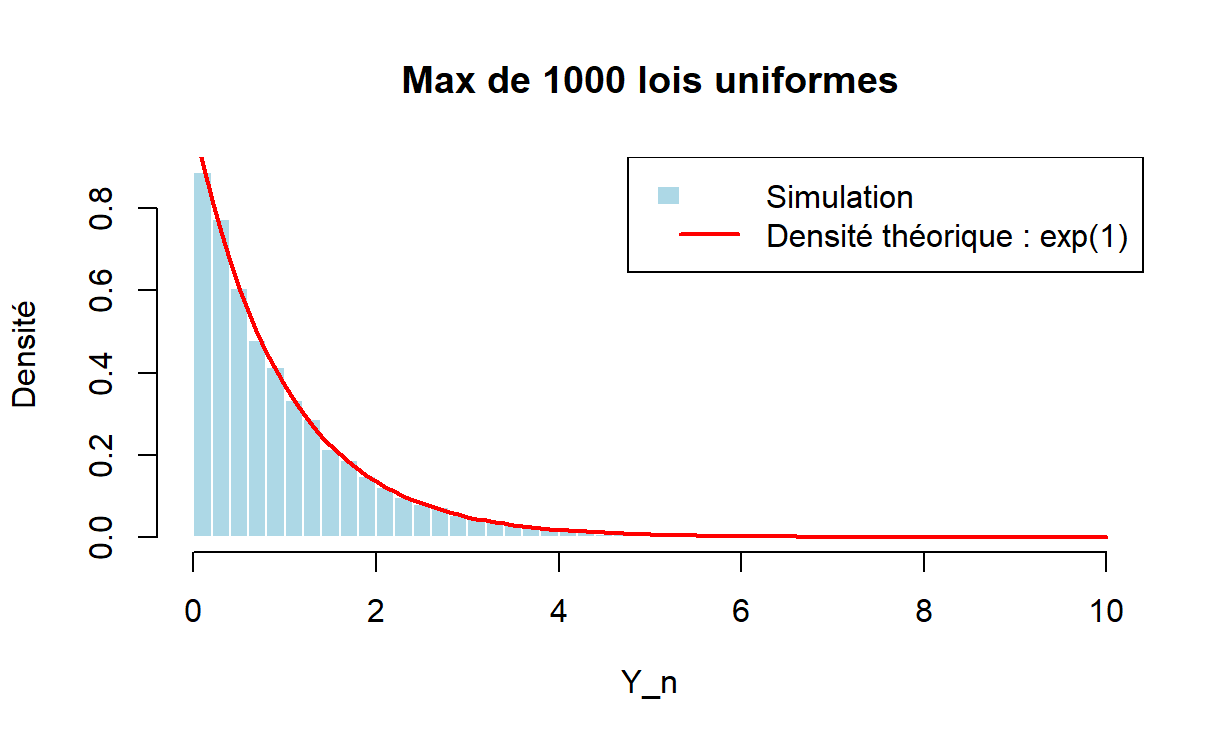
\includegraphics[scale=0.8]{./images/Max_Uniforme.png} 
\end{center}

\noindent Remarquons que l'on obtient une loi de Weibull, ce qui est logique au vu du fait que ce soit une loi à queue très légère, elle n'en a tout simplement pas car son support est borné.

\subsubsection{Loi exponentielle}
\noindent On considère une loi exponentielle de paramètre 1, la loi limite est une loi de Gumbel. Montrons que $a_n = 1 $ et $b_n = \log(n) $ conviennent. \\
\noindent En effet, soient $X_1, \dots, X_n$ des variables aléatoires iid de loi $\mathcal{E}(1)$. On a pour $ x \geq 0 $ :

\begin{align*}
	P(M_n \leq x) &= P(X_1 \leq x, \dots, X_n \leq x) \\
	&= (1-\exp(- x))^n
\end{align*}

\noindent Passons donc à la normalisation, posons $z=\frac{x-b_n}{a_n}$, on va utiliser le fait que $(1-\exp(- x))^n \xrightarrow[x \to +\infty]{} \exp(-n\exp(-x)) $. \\
\noindent Ainsi on veut choisir $b_n$ de telle sorte que $n \exp(-b_n) \xrightarrow[n \to +\infty]{} 1 $. D'où $b_n = \log(n)$. \\
\noindent On peut donc choisir $ a_n = 1$ afin d'avoir : 
\begin{align*}
	P(\frac{M_n - \log(n)}{1} \leq z) &= (1 - \exp(-(z+\log(n))))^n \\
	&= (1 - \frac{\exp(-z)}{n})^n 
\end{align*}

\noindent Et donc : $ (1 - \frac{\exp(-z)}{n})^n \xrightarrow[n \to +\infty]{} \exp(\exp(-z))$ \\

\noindent Ainsi, on a bien montré que $\frac{M_n - \log(n)}{1} \xrightarrow{\mathcal{L}} \text{Gumbel}(0,1) $ \\

\noindent On obtient alors numériquement le graphe suivant :

\begin{center}
	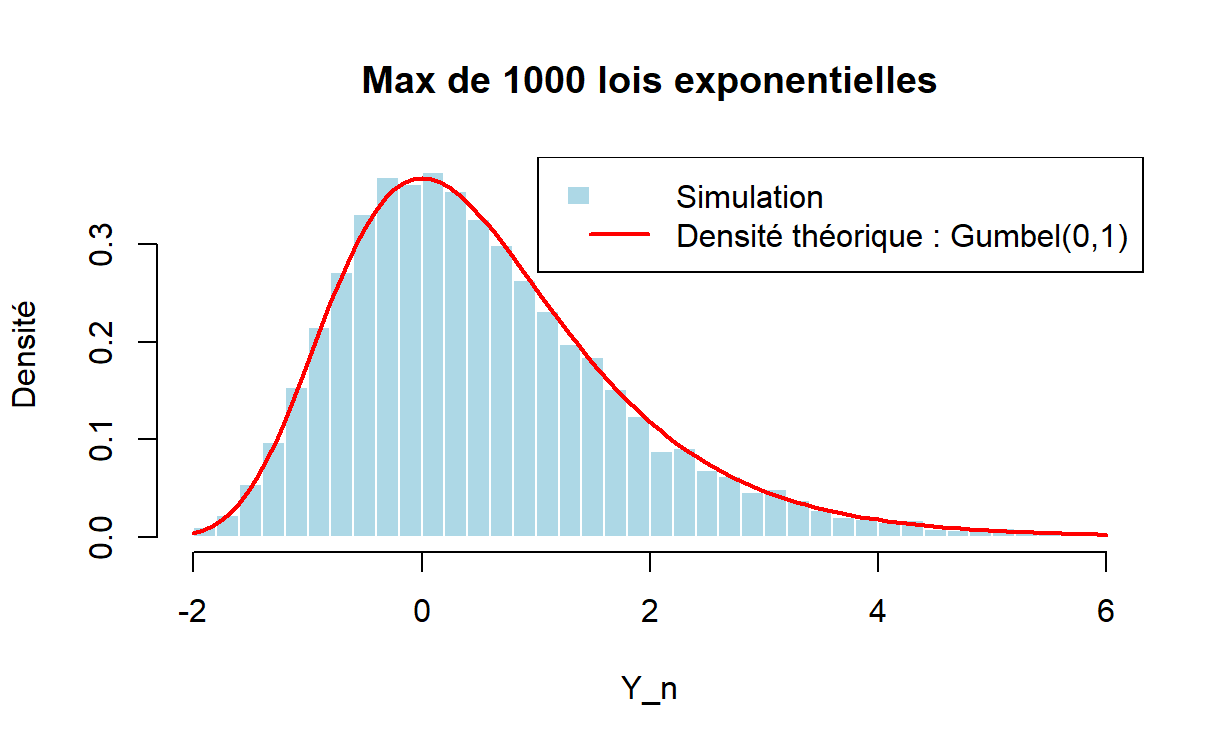
\includegraphics[scale=0.8]{./images/Max_Expo.png} 
\end{center}

\noindent Les valeurs de la loi exponentielle décroissent rapidement, on peut donc caractériser sa queue de distribution comme étant fine, on obtient donc une loi de Gumbel, ce qui était attendu.

\subsubsection{Loi normale}

\noindent Considérons maintenant une loi normale centrée réduite, on peut montrer que la loi limite est encore une fois une loi de Gumbel. Théoriquement, on peut démontrer que les paramètres généralisés suivants sont satisfaisants : $a_n = \frac{\log\left(\frac{4\log^2(2)}{\log^2\left(\frac{4}{3}\right)}\right)}{2\sqrt{2\log(n)}} $ et $b_n = \sqrt{2\log(n)} - \frac{\log(\log(n)) + \log\left(4\pi \log^2(2)\right)}{2\sqrt{2\log(n)}} $. (voir Gnedenko, \textit{On The Limiting Distribution of the Maximum Term in a Random Series}). \\

\noindent On obtient cette fois-ci le graphe suivant :

\begin{center}
	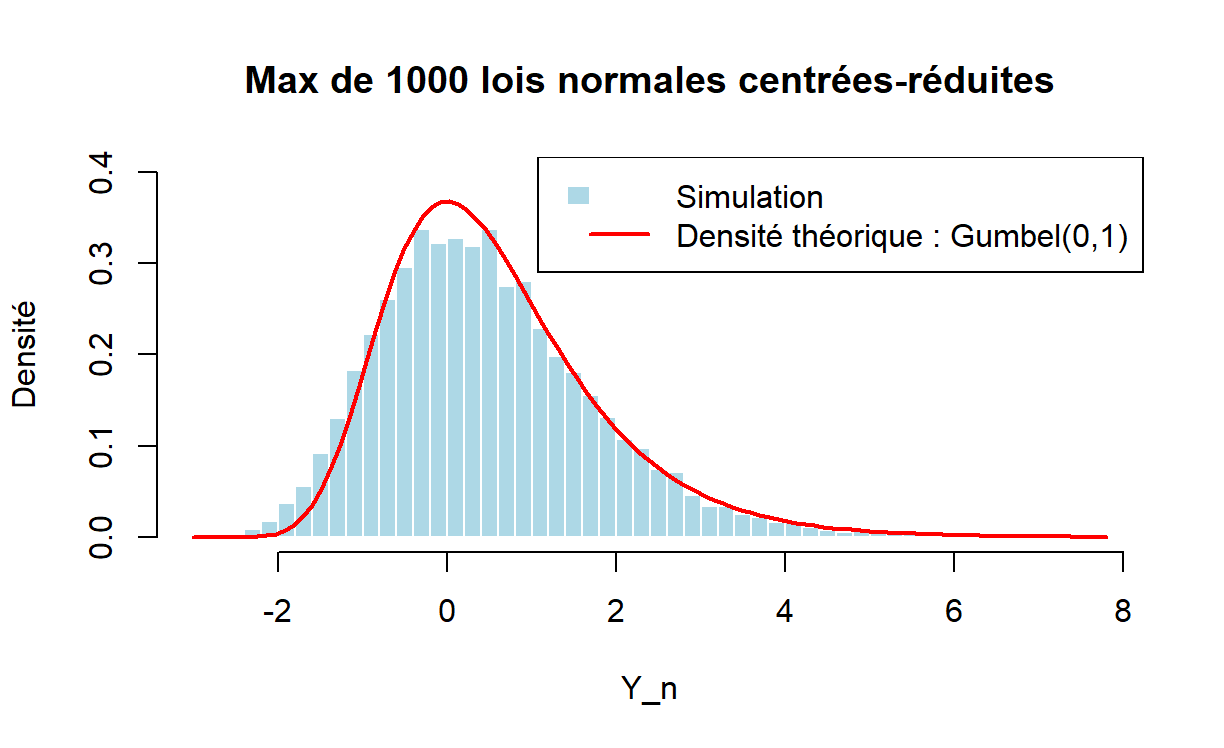
\includegraphics[scale=0.8]{./images/Max_Normale.png} 
\end{center}

\noindent Notons ainsi que l'on a la même loi limite que pour la loi exponentielle de paramètre 1, les graphes sont quasiment identiques.

\subsubsection{Loi de Cauchy}

\noindent Enfin, pour une loi de Cauchy (de paramètres 0 et 1 ici), la loi limite est une loi de Fréchet. Les coefficients suivants conviennent : $a_n = \pi $ et $b_n = n $. \\

\noindent Pour une loi de Cauchy, on sait que la fonction de répartition est donnée par $ F(x) = \frac{1}{2} + \frac{1}{\pi} \arctan(x) $. Donc, sa fonction de survie est $ \bar{F}(x) = 1 - F(x) = \frac{1}{2} - \frac{1}{\pi} \arctan(x) $. \\

\noindent Pour \( x \to +\infty \), on a le développement asymptotique suivant : $\arctan(x) = \frac{\pi}{2} - \frac{1}{x} + o\left(\frac{1}{x}\right) $. \\

\noindent Ainsi, on a $\bar{F}(x) \sim \frac{1}{\pi x} \quad \text{lorsque } x \to +\infty$. \\

\noindent Et donc la loi du maximum \( M_n \) s’écrit alors : $ \mathbb{P}(M_n \leq x) = F(x)^n \xrightarrow[n \to +\infty]{} \left(1 - \frac{1}{\pi x}\right)^n $


\noindent On cherche donc \( a_n > 0 \), \( b_n \) tels que : $ \mathbb{P}\left( \frac{M_n - b_n}{a_n} \leq z \right) \xrightarrow[n \to +\infty]{} \exp(-1/z) $ \\

\noindent Posons \( b_n = n \), \( a_n = \pi \). Il vient :

\[
\mathbb{P}\left( \frac{M_n - n}{\pi} \leq z \right) = \mathbb{P}\left( M_n \leq \pi z + n \right) \xrightarrow[n \to +\infty]{} \left(1 - \frac{1}{\pi(\pi z + n)}\right)^n
\]

\noindent En développant, on obtient : $\left(1 - \frac{1}{\pi(\pi z + n)}\right)^n \xrightarrow[n \to +\infty]{} \exp\left(- \frac{n}{\pi(\pi z + n)} \right)$

\noindent Donc : $\mathbb{P}\left( \frac{M_n - n}{\pi} \leq z \right) \xrightarrow[n \to +\infty]{} \exp\left(-\frac{1}{z} \right)$ \\

\noindent Ce qui montre que :
\[
\frac{M_n - n}{\pi} \xrightarrow[n \to +\infty]{\mathcal{L}} Z \sim \text{Fréchet}(1)
\]

\noindent Une simulation donne :

\begin{center}
	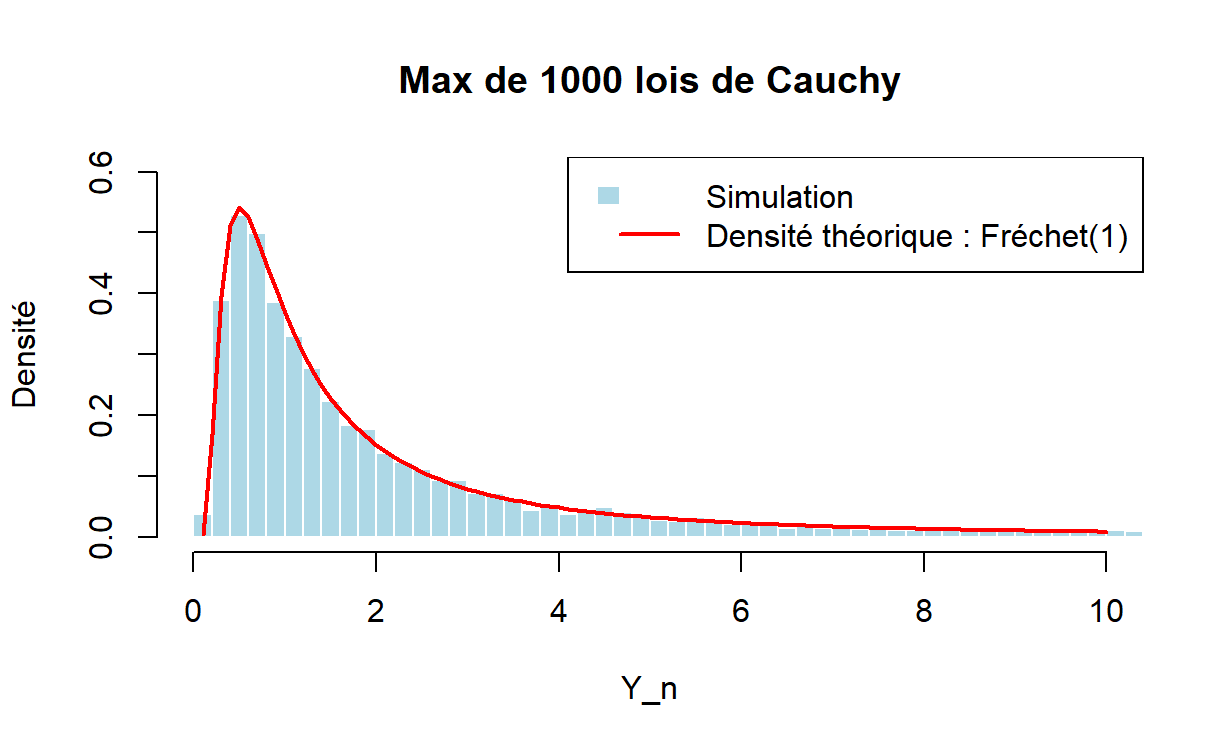
\includegraphics[scale=0.8]{./images/Max_Cauchy.png} 
\end{center}

\noindent Les valeurs extrêmes de la loi de Cauchy décroissent lentement, ce qui est caractéristique d'une loi à queue lourde. La simulation confirme donc que la loi limite est bien une loi de Fréchet comme nous l'avions vu théoriquement.

\section{Méthodes d'estimation de l'indice de valeurs extrêmes}
\noindent Dans cette section, nous cherchons à estimer le paramètre \(\gamma\) directement à partir des observations \(X_i\), sans nous limiter aux maxima \(M_n\), afin de tirer parti de l’ensemble des données.  
Nous nous concentrons sur deux approches non paramétriques classiques : les estimateurs de Hill et de Pickands. Ces méthodes reposent uniquement sur les statistiques d’ordre et sont particulièrement utilisées en pratique. D'autres estimateurs existent, notamment des versions généralisées ou des approches paramétriques basées sur la vraisemblance ou les moments, mais ils ne seront pas abordés ici. \\

\begin{definition}
On appelle \textit{statistique d'ordre} la permutation aléatoire de l'échantillon \(X_1, \dots, X_n\), qui ordonne les valeurs de l’échantillon par ordre croissant :

\[
X_{(1)} \leq X_{(2)} \leq \dots \leq X_{(n)}
\]
\end{definition}

\begin{definition}
On dit qu'une suite \((k_n)_{n \geq 1}\) d'entiers est intermédiaire si :

\[
\lim_{n \to \infty} k_n = \infty, \quad \lim_{n \to \infty} \frac{k_n}{n} = 0
\]

\end{definition}


\begin{definition}
On dit qu'un estimateur \(\hat{\gamma_{n}}\) est convergent s'il converge en probabilité vers \(\gamma\), soit :
\[
\lim_{n \to \infty} P(\lvert \hat{\gamma_{n}} - \gamma \rvert > \epsilon) = 0 \quad \forall \epsilon > 0
\]  
\end{definition}

\subsection{Estimateur de Pickands}
L’estimateur de Pickands est construit à partir de trois statistiques d’ordre d'un échantillon. Il constitue l’un des premiers estimateurs non paramétriques proposés pour estimer l’indice des valeurs extrêmes \(\gamma\). Son principal avantage réside dans le fait qu’il est valide quel que soit le domaine d’attraction de la loi sous-jacente. Il n'est donc pas restreint à une famille particulière de distributions et reste applicable dans un cadre très général.

Cependant, cet estimateur est connu pour être sensible à la taille de l’échantillon, en particulier au choix du paramètre intermédiaire \(k_n\). Cette dépendance peut induire une variabilité notable dans les estimations, notamment pour des échantillons de taille modeste, ce qui limite sa robustesse dans certaines situations pratiques.
\\
\\
\medskip
\begin{definition}
Soit \(X_1, \dots, X_n\) une suite de variables aléatoires i.i.d de loi \(F\), appartenant à l’un des domaines d’attraction des lois de valeurs extrêmes. On note \(X_{(1)} \leq X_{(2)} \leq \dots \leq X_{(n)}\) les statistiques d’ordre associées à l’échantillon. Soit \((k_n)_{n \geq 1}\) une suite intermédiaire.
L’estimateur de Pickands est défini par :
\[
\hat{\gamma}_{k_n,n} = \frac{1}{\ln(2)} \ln\left( \frac{X_{n-k_n+1,n} - X_{n-2k_n+1,n}}{X_{n-2k_n+1,n} - X_{n-4k_n+1,n}} \right)
\]
\end{definition}
\medskip
\noindent Cet estimateur repose sur le comportement asymptotique des grandes statistiques d’ordre. Plus précisément, sous l’hypothèse que la loi sous-jacente appartient au domaine d’attraction d’une loi extrême, la queue de la distribution peut être approchée localement par une fonction puissance. Ainsi, les rapports d’intervalles entre les grandes valeurs suivent une régularité qui dépend uniquement de l’indice de queue \(\gamma\). En prenant une combinaison logarithmique de ces rapports, on obtient une estimation directe de \(\gamma\).
\medskip
\begin{property}
Si \((k_n)_{n \geq 1}\) est une suite intermédiaire, alors :
\[
\hat{\gamma}_{k,n} \xrightarrow{\mathbb{P}} \gamma
\quad \text{lorsque } n \to \infty.
\]
\end{property}
\noindent De plus, sous des hypothèses régulières, telles que l’appartenance de la loi sous-jacente au domaine d’attraction d’une loi de valeur extrême et la condition que la suite $(k_n)_{n \geq 1}$ soit intermédiaire, l’estimateur de Pickands est asymptotiquement normal :
\[
\sqrt{k} \left( \hat{\gamma}_{k,n} - \gamma \right) \xrightarrow{\mathcal{L}} \mathcal{N}(0, \sigma^2(\gamma))
\]
où la variance asymptotique est donnée par :
\[
\sigma(\gamma) = \frac{\gamma \sqrt{2^{2\gamma + 1} + 1}}{2(2^{\gamma} - 1)\ln(2)}.
\]

\medskip
\noindent Cette formule théorique permet de construire des intervalles de confiance pour l’estimation de \(\gamma\), bien qu’en pratique la variance soit souvent estimée par simulation.

\subsubsection{Construction de l'estimateur de Pickands}

\noindent Afin de construire l'estimateur de Pickands, nous allons reprendre la proposition (2.3). Pour \(x,y > 0\) et \(y \neq 1\), la proposition est équivalente à :
\[
\lim_{t \to 0} \frac{U(tx) - U(t)}{U(ty) - U(t)} = 
\begin{cases} 
\frac{x^\gamma - 1}{y^\gamma - 1} & \text{si } \gamma \neq 0, \\
\frac{\log(x)}{\log(y)} & \text{si } \gamma = 0.
\end{cases}
\]
\newline

\begin{lemma}
Soit \(X_1, \dots, X_n\) des variables aléatoires indépendantes et de fonction de répartition \(F\).
Soit \(U_1, \dots, U_n\) des variables aléatoires indépendantes de loi uniforme \(\left[0,1\right]\). Alors \(F^{-1}(U_{(1)}), \dots, F^{-1}(U_{(n)})\) a même loi que \((X_{(1)}, \dots, X_{(n)})\).
\end{lemma}

\begin{proof}
admis
\end{proof}
\noindent
Ce résultat généralise un fait fondamental en probabilité selon lequel, si \(U \sim \mathcal{U}[0,1]\), alors \(F^{-1}(U) \sim F\). Ici, cette propriété est étendue au cas des statistiques d'ordre : la suite \((F^{-1}(U_{1,n}), \dots, F^{-1}(U_{n,n}))\) a même loi que \((X_{1,n}, \dots, X_{n,n})\). Cela justifie la construction d’estimateurs basés sur les quantiles empiriques, tels que l’estimateur de Pickands.
\\
\\
\noindent \textbf{Construction de l'estimateur de Pickands :}
\noindent La démonstration qui suit est adaptée du contenu présenté par Yoann (2019) sur la plateforme RPubs\footnote{Yoann, \textit{Estimateur de Hill – Illustration avec R}, consulté sur \url{https://rpubs.com/Yoann/499582}, en mars 2025.}.
\noindent Par la proposition précédente, pour $\gamma \in \mathbb{R}$ on a avec le choix $t = 2s$, $x = 2$ et $y = \frac{1}{2}$,
\[
\lim_{t \to \infty} \frac{U(t) - U(t/2)}{U(t/2) - U(t/4)} = 2^{\gamma}.
\]

\noindent En utilisant la croissance de $U$ qui se déduit de la croissance de $F$, on obtient
\[
\lim_{t \to \infty} \frac{U(t) - U(t_{c_1}(t))}{U(t_{c_1}(t)) - U(t_{c_2}(t))} = 2^{\gamma}
\]
dès que $\lim_{t \to \infty} c_1(t) = \frac{1}{2}$ et $\lim_{t \to \infty} c_2(t) = \frac{1}{4}$. Il reste donc à trouver des estimateurs pour $U(t)$.
\\
\\
Soit $k_n,$ pour $ n \geq 1$ une suite d’entiers telle que $1 \leq k_n \leq \frac{n}{4}$ et $\lim_{n \to \infty} \frac{k_n}{n} = 0$ et $\lim_{n \to \infty} k_n = \infty$.
\\
Soit $(V_{1,n},\dots,V_{n,n})$ la statistique d’ordre d’un échantillon de variables aléatoires indépendantes de loi de Pareto. On note $F_V(x) = 1 - x^{-1}, x \geq 1$.
\\
\\
\noindent On déduit avec certains résultats de bases liés à $(V_{1,n},\dots,V_{n,n})$ que les suites
\[
\frac{k_n}{n} V_{n-k_n+1,n}, \quad \frac{2k_n}{n} V_{n-2k_n+1,n}, \quad \frac{4k_n}{n} V_{n-4k_n+1,n}
\]
pour \(n \geq 1\) convergent en probabilité vers 1.

\noindent On en déduit en particulier, les convergences en probabilité suivantes :
\[
V_{n-k_n+1,n}  \to \infty, \quad \frac{V_{n-2k_n+1,n}}{V_{n-k_n+1,n}} \to \frac{1}{2}, \quad \frac{V_{n-4k_n+1,n}}{V_{n-k_n+1,n}} \to \frac{1}{4}.
\]

\noindent Donc la convergence suivante a lieu en probabilité :
\[
\frac{U(V_{n-k_n+1,n}) - U(V_{n-2k_n+1,n})}{U(V_{n-2k_n+1,n}) - U(V_{n-4k_n+1,n})} \to 2^{\gamma}.
\]

\noindent Remarquons que si $x \geq 1$, alors $U(x) = F^{-1}(F_V(x))$. On a donc
\[
(U(V_{1,n}), \dots, U(V_{n,n})) = (F^{-1}(F_V(V_{1,n})), \dots, F^{-1}(F_V(V_{n,n}))).
\]

\noindent Or, \(F_V\) est la fonction de répartition de la loi de Pareto. \newline
On déduit de la croissance de $F_V$ que $(F^{-1}(F_V(V_{1,n})),\dots, F^{-1}(F_V(V_{n,n})))$ a la même loi qu’une suite de $n$ variables aléatoires uniformes sur $[0,1]$ indépendantes. 

\noindent Et d'après le lemme précédent, le vecteur aléatoire $(F^{-1}(F_V(V_{1,n})),\dots, F^{-1}(F_V(V_{n,n})))$ a la même loi que $(X_1,\dots,X_n)$. \\

\noindent Donc la variable aléatoire \(\frac{U(V_{n-k_n+1,n}) - U(V_{n-2k_n+1,n})}{U(V_{n-k_n+1,n}) - U(V_{n-4k_n+1,n})}\) a la même loi que :

\[
\frac{X_{n-k_n+1,n} - X_{n-2k_n+1,n}}{X_{n-k_n+1,n} - X_{n-4k_n+1,n}}
\]

\noindent Ainsi cette quantité converge en loi vers $2^{\gamma}$ quand $n$ tend vers l’infini.

\subsubsection{Représentation graphique de l’estimateur de Pickands}

\noindent Pour mieux comprendre le comportement de l’estimateur de Pickands dans différents contextes, nous l’appliquons à des données simulées qui sont les mêmes que dans la partie 3, c'est à dire : Pareto, Exponentielle, Uniforme et Cauchy. Ces lois sont choisies pour représenter les trois domaines d’attraction des lois de valeurs extrêmes.

\noindent Chaque échantillon comporte $n = 100000$ observations, et la représentation graphique est faite en fonction de $k$, où \(k\) représente le nombre de plus grandes valeurs utilisées pour estimer l’indice de queue \(\gamma\).

\begin{figure}[H]
    \centering
    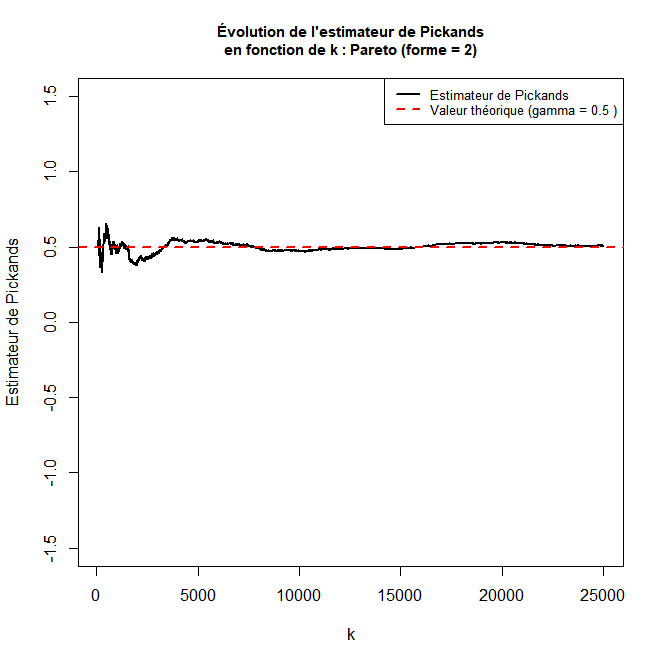
\includegraphics[width=0.6\textwidth]{./Evolution des estimateurs/pickands/estimateur_pickands_pareto.png}
    \caption{Estimateur de Pickands appliqué à la loi de Pareto ($\gamma = 0.5$)}
\end{figure}
\noindent Tout d'abord, pour la loi de Pareto, nous remarquons que l'estimateur de Pickands converge rapidement et de manière stable vers la valeur théorique \(\gamma = 0.5\), dès que \(k\) devient raisonnablement grand. Cela confirme la bonne performance de l’estimateur pour les lois à queue lourde. On observe cependant une légère variabilité pour les très petites valeurs de \(k\), car dans ce cas, l’estimation repose sur un nombre insuffisant de données, ce qui la rend plus sensible aux fluctuations aléatoires.

\begin{figure}[H]
    \centering
    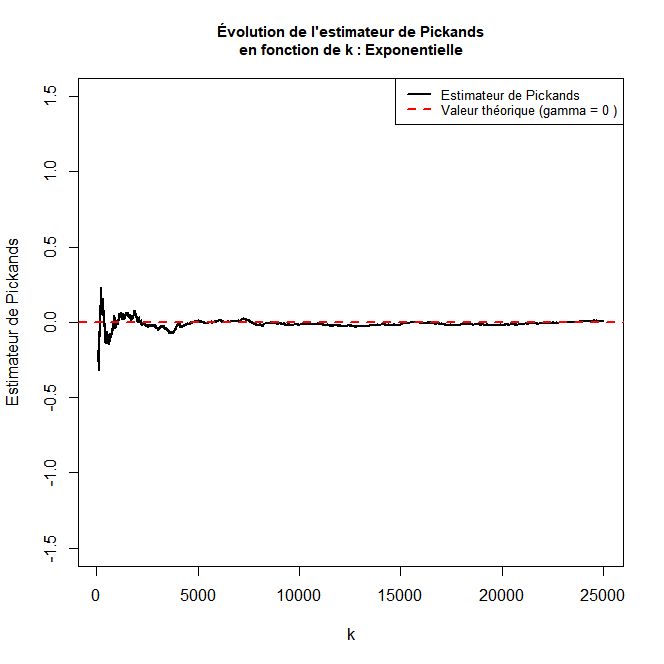
\includegraphics[width=0.6\textwidth]{./Evolution des estimateurs/pickands/estimateur_pickands_exponentielle.png}
    \caption{Estimateur de Pickands appliqué à la loi Exponentielle ($\gamma = 0$)}
\end{figure}
\noindent Dans le cas de la loi exponentielle, qui appartient au domaine d'attraction de Gumbel, l’estimateur de Pickands se stabilise rapidement autour de \(\gamma = 0\). Ce comportement est conforme aux attentes théoriques, puisque pour les distributions à queue exponentielle, l’indice de queue est effectivement nul.

\begin{figure}[H]
    \centering
    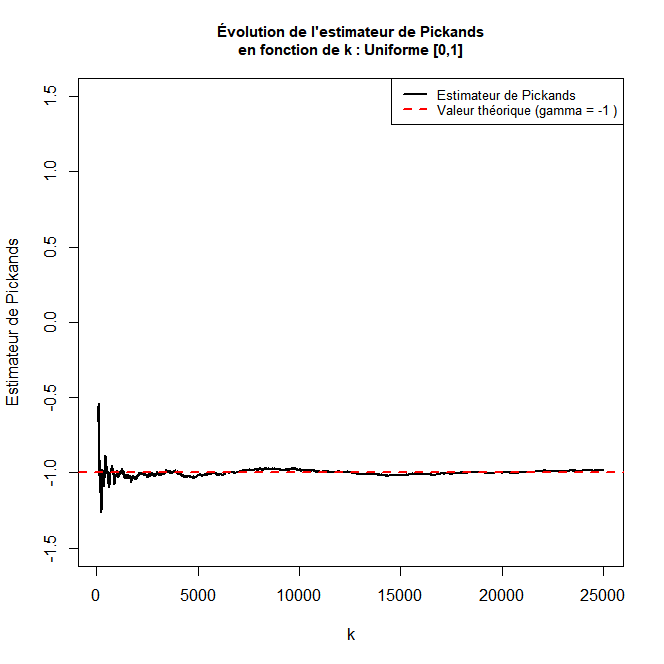
\includegraphics[width=0.6\textwidth]{./Evolution des estimateurs/pickands/estimateur_pickands_uniforme.png}
    \caption{Estimateur de Pickands appliqué à la loi Uniforme ($\gamma = -1$)}
\end{figure}
\noindent Avec la loi uniforme, dont le support est borné, l’estimateur converge vers $\gamma = -1$, ce qui est cohérent avec la théorie. On observe une plus grande variabilité dans les faibles valeurs de $k$, mais une convergence raisonnablement bonne lorsque $k$ augmente.


\begin{figure}[H]
    \centering
    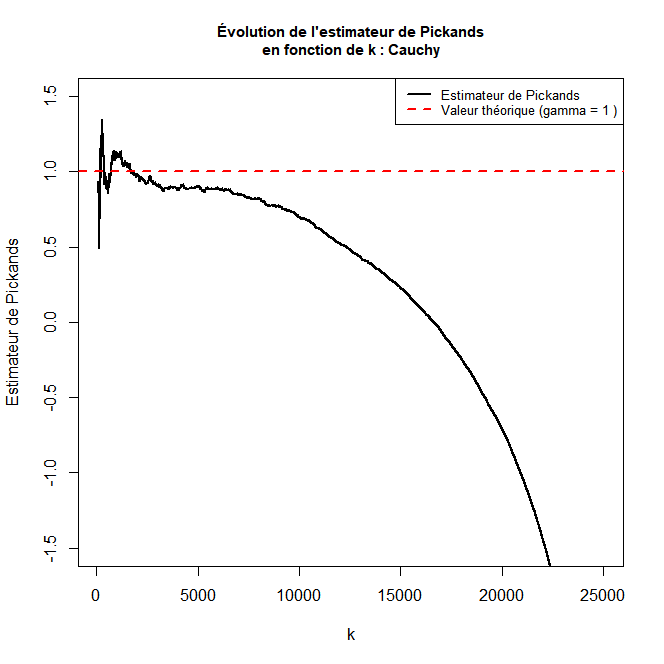
\includegraphics[width=0.6\textwidth]{./Evolution des estimateurs/pickands/estimateur_pickands_cauchy.png}
    \caption{Estimateur de Pickands appliqué à la loi de Cauchy ($\gamma = 1$)}
\end{figure}
\noindent La loi de Cauchy, caractérisée par une queue extrêmement lourde, induit un comportement plus instable de l’estimateur de Pickands. Pour les faibles valeurs de \(k\), l’estimateur est très variable. On observe un plateau autour de \(\gamma = 1\) dès \(k \approx 5000\), ce qui suggère une estimation correcte dans cette zone. Toutefois, lorsque \(k\) devient trop grand (au-delà de \(k \approx 10000\)), l’estimateur commence à décroître, indiquant une perte de précision. Ce phénomène illustre la sensibilité de l’estimateur de Pickands au choix de \(k\), en particulier pour les lois à queue très lourde : l’inclusion de données moins extrêmes peut introduire un biais significatif.

\vspace{0.5cm}

\noindent Ainsi, ces résultats illustrent bien les limites de l’estimateur de Pickands : si \(k\) est trop petit, on observe une forte variance, tandis que si \(k\) est trop grand, l’estimation est biaisée car elle intègre des observations non extrêmes. D’un point de vue théorique, la validité asymptotique de l’estimateur repose sur les conditions suivantes : \(k \to \infty\) et \(k/n \to 0\) lorsque \(n \to \infty\). Cela signifie qu’on doit considérer suffisamment de valeurs extrêmes, tout en veillant à ce que \(k\) reste petit devant \(n\). Dans cette optique, nous limitons volontairement \(k\) à \(n/4\) dans nos simulations, afin de respecter ce cadre théorique et d’éviter que l’estimation ne soit dégradée.


\subsection{Estimateur de Hill}

\noindent Cet estimateur a été introduit par Hill en 1975 dans le but d’estimer, de manière non paramétrique, le paramètre de queue des lois appartenant au domaine d’attraction de Fréchet. Il offre une estimation de l’indice de queue généralement plus efficace que celle fournie par l’estimateur de Pickands. La construction de cet estimateur repose sur l’utilisation des $k_n$ plus grandes statistiques d’ordre de l’échantillon.



\subsubsection{La construction de l’estimateur de Hill}
\noindent Dans le cadre de l'analyse des valeurs extrêmes, l'estimation de l'indice de queue \(\gamma\) est cruciale pour comprendre le comportement des queues de distribution. L'estimateur de Hill est une méthode largement utilisée pour estimer cet indice de queue.

\noindent Nous présentons ci-dessous une démonstration classique de la construction de cet estimateur, en nous inspirant du mémoire de Bouazza (2018)\footnote{I. Bouazza, \textit{Estimation non-paramétrique des quantiles extrêmes conditionnels}, Mémoire de Master, Université de Saïda - Dr Moulay Tahar, 2018.}.
\noindent Soient \(\alpha_n\) et \(\beta_n\) deux suites de nombres positifs. La construction de l'estimateur de Hill repose sur une relation fondamentale entre les quantiles d’une distribution à queue lourde appartenant au domaine d’attraction de Fréchet. Cette relation est donnée par :

\[
    q_{\beta_n} \simeq q_{\alpha_n} \left( \frac{\alpha_n}{\beta_n} \right)^{\gamma}.
\]

\noindent Ici, \(q_{\alpha}\) représente le quantile d'ordre \(\alpha\) de la distribution, et \(\gamma\) est l'indice de queue que nous cherchons à estimer. Cette relation exprime que le quantile d'ordre \(\beta_n\) peut être approximé par le quantile d'ordre \(\alpha_n\) multiplié par un facteur dépendant de \(\gamma\).

\noindent Pour obtenir l'estimateur de Hill, nous commençons par prendre le logarithme des deux côtés de l'équation du dessus. Nous obtenons :

\[
\log(q_{\beta_n}) - \log(q_{\alpha_n}) \simeq \gamma \log\left( \frac{\alpha_n}{\beta_n} \right).
\]

\noindent En posant $\alpha_n = k_n/n$, où \(k_n\) est un nombre d'observations extrêmes que nous considérons, et en prenant plusieurs valeurs pour \(\beta_n\), avec \(\beta_n = i/n\) pour \(i = 1, \ldots, k_n - 1\) et \(\beta_n < \alpha_n\), nous obtenons :

\[
\log(q_{i/n}) - \log(q_{k_n/n}) \simeq \gamma \log(k_n/i).
\]

\noindent Ensuite, nous estimons les quantiles par leurs équivalents empiriques, c'est-à-dire les statistiques d'ordre de l'échantillon. Cela conduit à :

\[
\log(X_{n - i + 1, n}) - \log(X_{n - k_n + 1, n}) \simeq \gamma \log(k_n / i).
\]

\noindent En sommant sur \(i = 1, \ldots, k_n - 1\), nous obtenons :

\[
\gamma = \frac{\sum_{i=1}^{k_n - 1} \log(X_{n - i + 1, n}) - \log(X_{n - k_n + 1, n})}{\sum_{i=1}^{k_n - 1} \log(k_n / i)}.
\]

\noindent Le dénominateur peut être réécrit comme \(\log(k_n^{k_n - 1}/(k_n - 1)!)\). En utilisant la formule de Stirling, nous trouvons que ce dénominateur est équivalent à \(k_n\) au voisinage de l'infini. Cela nous permet d'obtenir l'estimateur de Hill.

\noindent Soit $(k_n)_{n \geq 1}$ une suite d'entiers avec $1 \leq k_n \leq n$, l’estimateur de Hill est défini par :

\[
\hat{\gamma}^{H}_{k_n} = \frac{1}{k_n - 1} \sum_{i=1}^{k_n - 1} \log(X_{n - i + 1, n}) - \log(X_{n - k_n + 1, n}).
\]

\noindent L’estimateur de Hill satisfait la propriété de consistance faible. Plus précisément, si $(k_n)_{n \geq 1}$ est une suite intermédiaire, alors l’estimateur $\hat{\gamma}^{H}_{k_n}$ converge en probabilité vers le paramètre de queue $\gamma$, c’est-à-dire :
\[
\hat{\gamma}^{H}_{k_n} \xrightarrow{\mathbb{P}} \gamma.
\]

\begin{remark}
	Dans la pratique, déterminer une valeur appropriée pour le paramètre $k_n$, c’est-à-dire le nombre de plus grandes observations à retenir, constitue une étape délicate. Il faut en effet trouver un compromis entre la variance et le biais : utiliser suffisamment de données pour obtenir une estimation fiable, tout en s’assurant que ces données proviennent bien de la queue de la distribution. Diverses approches ont été développées dans la littérature pour guider ce choix.
\end{remark}

\subsubsection{Comportement empirique de l’estimateur de Hill}
\noindent Pour analyser le comportement de l’estimateur de Hill, nous l’appliquons à des échantillons simulés de taille \(n = 40000\), issus de plusieurs distributions : la loi de Lévy, la loi exponentielle, la loi uniforme sur \([0,1]\), et la loi de Cauchy. Ces distributions permettent d’explorer les trois domaines d’attraction des lois de valeurs extrêmes.
Il est important de noter que l’estimateur de Hill est conçu spécifiquement pour les lois à queue lourde, appartenant au domaine d’attraction de Fréchet (\(\gamma > 0\)). On ne s’attend donc pas à obtenir de bonnes performances pour des lois comme l’exponentielle ou l’uniforme, qui ne satisfont pas cette condition.
Les figures suivantes présentent l’évolution de l’estimateur de Hill en fonction de \(k\), le nombre de plus grandes valeurs utilisées. La ligne rouge indique la valeur théorique de \(\gamma\), tandis que la courbe noire représente l’estimation, accompagnée d’une bande de confiance à 95\%.
\begin{figure}[H]
    \centering
    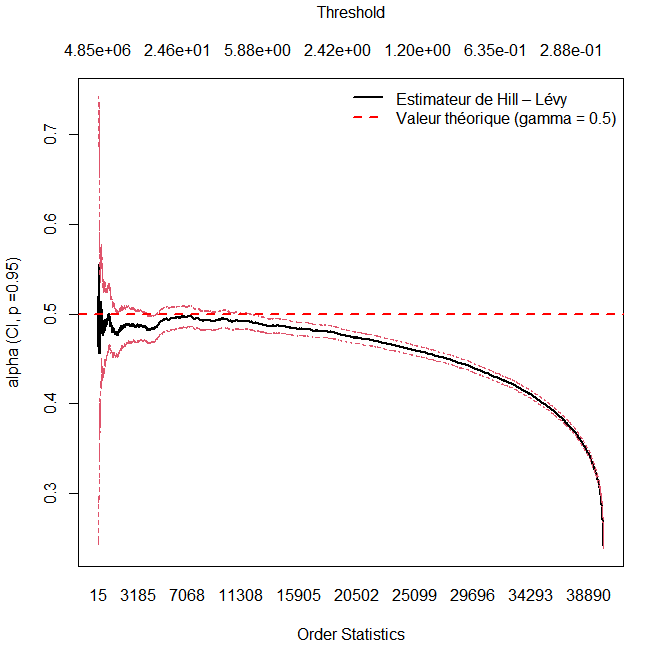
\includegraphics[width=0.55\textwidth]{./Evolution des estimateurs/hill/estimateur_hill_levy.png}
    \caption{Estimateur de Hill appliqué à la loi de Lévy ($\gamma = 0.5$)}
\end{figure}
\noindent La loi de Lévy est une loi à queue lourde appartenant au domaine d’attraction de Fréchet. Sa densité de probabilité est donnée par :

\[
f(x; \mu, c) =
\begin{cases}
\sqrt{\dfrac{c}{2\pi}} \dfrac{1}{(x - \mu)^{3/2}} \exp\left(-\dfrac{c}{2(x - \mu)}\right), & \text{si } x > \mu, \\
0, & \text{sinon.}
\end{cases}
\]

où \(\mu \in \mathbb{R}\) est un paramètre de position et \(c > 0\) un paramètre d’échelle. Cette loi est caractérisée par une forte asymétrie et une variance infinie.

\noindent Sur le graphique, on observe que l’estimateur de Hill converge globalement vers la valeur théorique \(\gamma = 0.5\), ce qui est attendu pour une loi à queue lourde. Cette convergence devient plus stable lorsque \(k\) atteint des valeurs modérées. Toutefois, lorsque \(k\) devient trop grand, on remarque une détérioration progressive de l’estimation : cela s'explique par l’inclusion d’observations moins extrêmes, qui introduisent un biais dans le calcul de l’estimateur.
\begin{figure}[H]
    \centering
    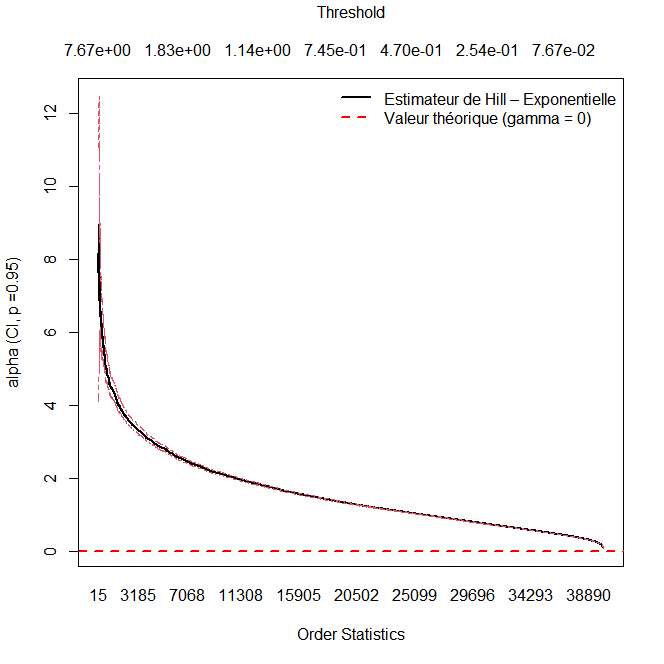
\includegraphics[width=0.55\textwidth]{./Evolution des estimateurs/hill/estimateur_hill_exponentielle.png}
    \caption{Estimateur de Hill appliqué à la loi exponentielle ($\gamma = 0$)}
\end{figure}
\noindent La loi exponentielle appartient au domaine de Gumbel, avec un indice de queue nul. L’estimateur de Hill n’est pas conçu pour ce cas, ce que montre bien le graphique : les valeurs estimées sont nettement surestimées et décroissent lentement sans atteindre la valeur théorique. Ce comportement traduit l’inadéquation de Hill pour ce type de loi.

\begin{figure}[H]
    \centering
    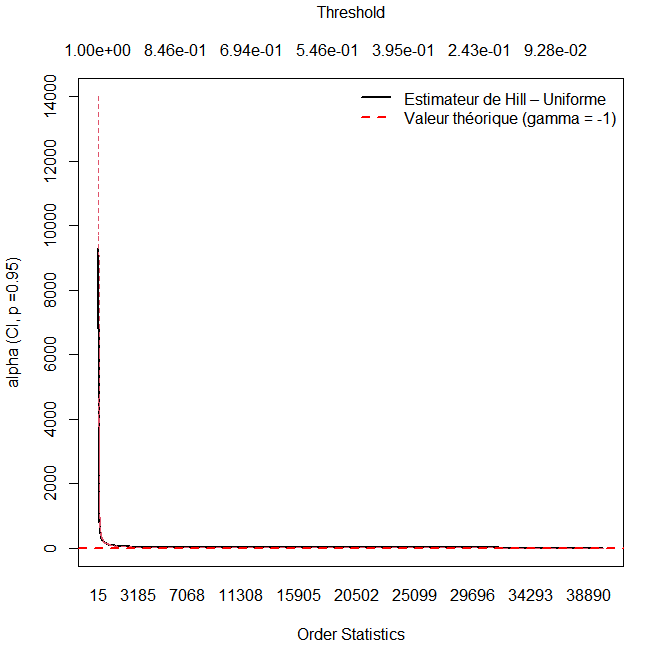
\includegraphics[width=0.55\textwidth]{./Evolution des estimateurs/hill/estimateur_hill_uniforme.png}
    \caption{Estimateur de Hill appliqué à la loi uniforme ($\gamma = -1$)}
\end{figure}
\noindent La loi uniforme a un support borné et un indice théorique de \(\gamma = -1\), ce qui sort du domaine d’application de Hill, qui suppose \(\gamma > 0\). L’estimateur produit ici des résultats très instables et incohérents, confirmant qu’il ne doit pas être utilisé sur ce type de distribution.

\begin{figure}[H]
    \centering
    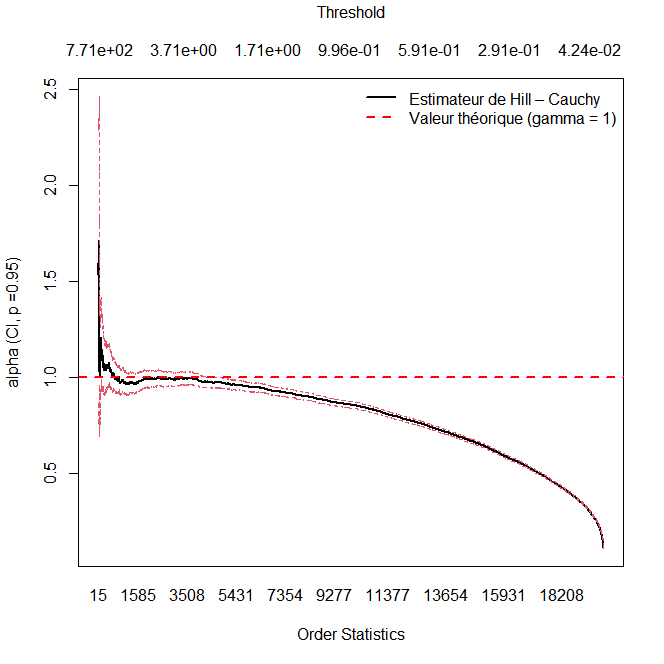
\includegraphics[width=0.55\textwidth]{./Evolution des estimateurs/hill/estimateur_hill_cauchy.png}
    \caption{Estimateur de Hill appliqué à la loi de Cauchy ($\gamma = 1$)}
\end{figure}
\noindent La loi de Cauchy, avec un indice $\gamma = 1$, appartient au domaine de Fréchet. L’estimateur fonctionne bien pour de faibles valeurs de $k$, avec une estimation proche de la valeur théorique. On observe un plateau autour de $k = 3000-4000$, indiquant une estimation stable dans cette plage. Cependant, dès que $k$ devient trop grand, la courbe chute, signe d’un biais induit par les valeurs non extrêmes. Cela illustre la sensibilité de l’estimateur au choix du seuil, similaire à ce qui est observé avec l'estimateur de Pickands. \\
\noindent Ainsi, ces résultats montrent que l’estimateur de Hill est très dépendant du choix du paramètre \(k\), et de la nature de la distribution. Un compromis est nécessaire entre biais (si \(k\) est trop grand) et variance (si \(k\) est trop petit), pour garantir une estimation fiable.


\section{Méthode des maxima par blocs}

\noindent L'approche des maxima par blocs (en anglais Blocks Maxima) consiste à diviser les n observations en N blocs de taille k. Concrètement, la suite $X_1, ..., X_n$ est divisée en N blocs, le premier bloc est $X_1, ..., X_k$, le second $X_{k+1}, ..., X_{2k}$, etc. On obtient ainsi une suite de maxima $M_1, ..., M_n$ définis sur chacun des blocs.\\
\noindent En général, on considère une période temporelle, comme une journée ou bien une année pour refléter le sens des observations.  \\
\noindent On peut alors déterminer la loi limite des maxima, en vertu du théorème de Fisher-Tippett-Gnedenko c'est une distribution GEV classique de la forme :
\[
G_{\mu,\sigma,\gamma}(x)
\;=\;
\exp\!\Bigl\{-\bigl[1 + \gamma\,u\bigr]^{-1/\gamma}\Bigr\}.
\]

\noindent De la même manière que ce que l'on avait sans les blocs, il faut alors déterminer les valeurs des paramètres en les approximant par des méthodes comme le maximum de vraisemblance. Des auteurs comme Ferreira et de Haan (2006 et 2015) ont alors démontré l'existence d'estimateurs pertinents pour cette méthode, nommés PWM (pour "probability weighted moment"). Pour les définir, on part de la statistique suivante, soient $X_{1,k}, ..., X_{k,k}$ les observations ordonnées du bloc $X_1, ..., X_k$, on définit :
\[
\beta_r = \frac{1}{k} \sum_{i=1}^{k} \frac{(i-1)...(i-r)}{(k-1)...(k-r)} X_{i,k} ~ \text{ pour $r = 1,2,3,...,k>r $}
\] \\
\noindent A partir de $\beta_r$, on peut ensuite définir les trois estimateurs PVM suivants pour $\gamma, a_n$ et $b_n$ qui possèdent de bonnes propriétés asymptotiques sous certaines conditions ($\Gamma$ est la fonction gamma d'Euler). \\

\noindent Pour $\gamma$ : $\hat{\gamma}_{k,m}$ est solution de $\frac{3\hat{\gamma}_{k,m} - 1}{2\hat{\gamma}_{k,m} - 1} = \frac{3\beta_2 - \beta_0}{2\beta_1 - \beta_0} $ \\
\noindent Pour $a_n$ : $\hat{a}_{k,m} = \frac{\hat{\gamma}_{k,m}}{2\hat{\gamma}_{k,m} - 1} \cdot \frac{2\beta_1 - \beta_0}{\Gamma(1 - \hat{\gamma}_{k,m})}$ \\
\noindent Pour $b_n$ : $\hat{b}_{k,m} = \beta_0 + \hat{a}_{k,m} \cdot \frac{1 - \Gamma(1 - \hat{\gamma}_{k,m})}{\hat{\gamma}_{k,m}}$ \\

\noindent Cette approche possède tout de même un défaut car lorsque l'on prend le maximum sur un bloc, on fait potentiellement disparaître des valeurs élevées, on perd des données intéressantes.

\subsection{Quantile de retour}

\noindent En pratique, on cherche une valeur qui donnerait une certaine confiance quand à l'apparition
de données la depassant. Dans le cas d'une distribution à queue bornée il suffit de prendre la bornes supérieure de la distribution.
\\
Or, dans le cas d'une distribution à queue lourde et exponentiel ce n'est pas possible. On introduit alors la notion de \textbf{quantile de retour} qui est une valeur que l'on dépasse en moyenne une fois tous les T ans (\textit{Séminaire CNAM 2019}).
\\
On pose $z_T$ cette quantité, et elle est solution de l'équation suivante :
\[
P\bigl(M \le z_T\bigr)
\;=\;
G_{\mu,\sigma,\gamma}(z_T)
\;=\;
1 - \frac{1}{T},
\]
où \(G_{\mu,\sigma,\gamma}\) est la fonction de répartition de la GEV. En résolvant cette équation que l'on admet, on obtient
\[
z_T =
\begin{cases}
\displaystyle
\mu \;+\;\frac{\sigma}{\gamma}\Bigl[(-\ln(1 - 1/T))^{-\gamma} - 1\Bigr],
&\gamma \neq 0,\\[1em]
\displaystyle
\mu \;-\;\sigma\,\ln\bigl(-\ln(1 - 1/T)\bigr),
&\gamma = 0.
\end{cases}
\]
\\
\\
\section{Méthode des excès}

\noindent La méthode des excès, également appelée approche par dépassement de seuil (en anglais \textit{Peaks Over Threshold}, ou POT), a été introduite par Pickands en 1975. Elle constitue une alternative à l’approche classique par blocs pour modéliser les phénomènes extrêmes.

\noindent Le principe est de ne conserver que les observations excédant un seuil élevé \( u \). Si ce seuil est bien choisi la distribution des excès définis par :
\[
Y_i = X_i - u \quad \text{pour} \quad X_i > u
\]
peut être approximée par une distribution de Pareto généralisée (GPD).

\medskip
\noindent Cette approche repose sur un résultat fondamental de Balkema et de Haan (1974), et de Pickands (1975), selon lequel, pour une grande classe de lois de probabilité \(F\), la loi des excès conditionnels au-delà d’un seuil élevé converge vers une loi de Pareto généralisée lorsque le seuil \(u\) tend vers la borne supérieure de \(F\).

\medskip
\noindent Formellement, on considère une suite de variables aléatoires i.i.d. \(X_1, \dots, X_n\) de fonction de répartition \(F\), et \(x_F\) le point terminal de \(F\). Pour tout seuil \(u < x_F\), on définit la fonction de répartition des excès par :

\[
F_u(x) := \mathbb{P}(X - u \leq x \mid X > u) = \frac{F(x + u) - F(u)}{1 - F(u)},
\quad \text{pour } 0 \leq x \leq x_F - u.
\]

\noindent Et sa version en fonction de survie :
\[
\overline{F}_u(x) := \mathbb{P}(X - u > x \mid X > u) = \frac{\overline{F}(x + u)}{\overline{F}(u)}.
\]

\noindent Lorsque le seuil \(u\) est suffisamment élevé, \(F_u\) peut être bien approchée par une distribution de Pareto généralisée \(H_{\gamma, \beta(u)}\), définie comme suit :
\[
H_{\gamma, \beta}(y) =
\begin{cases}
1 - \left(1 + \dfrac{\gamma y}{\beta}\right)^{-1/\gamma}, & \text{si } \gamma \neq 0, \\
1 - \exp\left(-\dfrac{y}{\beta}\right), & \text{si } \gamma = 0,
\end{cases}
\]
avec \( y \geq 0 \), sous la condition \(1 + \gamma y/\beta > 0\). Le paramètre \(\beta > 0\) représente l’échelle et \(\gamma\) le paramètre de forme (indice de queue).

\medskip
\begin{example}
Soit \(F(x) = 1 - e^{-x}\) la loi exponentielle standard. On a pour tout \(y > 0\) :

\[
\mathbb{P}(X - u > y \mid X > u) = \frac{e^{-(u + y)}}{e^{-u}} = e^{-y}.
\]
On retrouve donc une loi exponentielle, qui correspond à une GPD avec \(\gamma = 0\) et \(\beta = 1\). Cela montre que l’exponentielle est un cas particulier de GPD.
\end{example}

\begin{theorem}

Le résultat central qui justifie l’utilisation de la GPD pour modéliser les excès est le suivant :

\begin{quote}
\noindent Soit \(F\) une fonction de répartition appartenant au domaine d’attraction d’une loi de valeur extrême. Alors, lorsque \(u \to x_F\), il existe une fonction \(\beta(u)\) telle que :
\[
\sup_{0 \leq x \leq x_F - u} \left| F_u(x) - G_{\gamma, \beta(u)}(x) \right| \to 0.
\]
\end{quote}
\end{theorem}
\noindent Autrement dit, plus le seuil \(u\) est élevé, plus la loi des excès au-dessus de ce seuil est bien approchée par une GPD.
\medskip
\noindent Cette propriété est essentielle en statistique des valeurs extrêmes, car elle permet d’exploiter pleinement les données situées dans les queues de distribution, sans se limiter au maximum d’un bloc.
\newpage
\section{Application sur des données réelles}
\subsection{Description des données}

\noindent Afin d'illustrer les méthodes d'estimation de l'indice de valeurs extrêmes, nous allons appliquer ces techniques sur des données réelles.
Nous allons utiliser les données du package $ismev$ de R. Plus précisément celui de rain et de danish. Ils contienent respectivement les données de pluie journalière en Angleterre de 1914 à 1962 et 
les montants des grands sinistres d'incendie survenus au Danemark entre 1980 et 1990 (Données issue du package \textbf{ismev} de R).
\\
\\
L'objectif sur ces données est de savoir s'il existe et le cas échéant de le calculer, une valeur tel qu'à l'avenir on la dépasse rarement tout en restant raisonable. C'est exactement ce que fait le quantile de retour.
\\
\\
Concernant les données de pluie, on dispose de $17531$ données qui prennent des valeurs entre $0$ et $86,6$. On observe un moyenne de $3,476$ et une médiane de $0,5$.
\\
On remarque de plus que les données sont fortement concentrées autour de 0.
Il est alors raisonnable de penser qu'après estimation, on va obtenir une valeur de gamma positive ou nulle. En effet, il n'apparait pas de cassure dans la distribution des données.
De plus, les données prennent des valeurs grandes mais perdent rapidement en densité pour celle-ci. Ce qui suggèrerait une valeur de gamma proche de $0$ et positive.

\begin{center}
	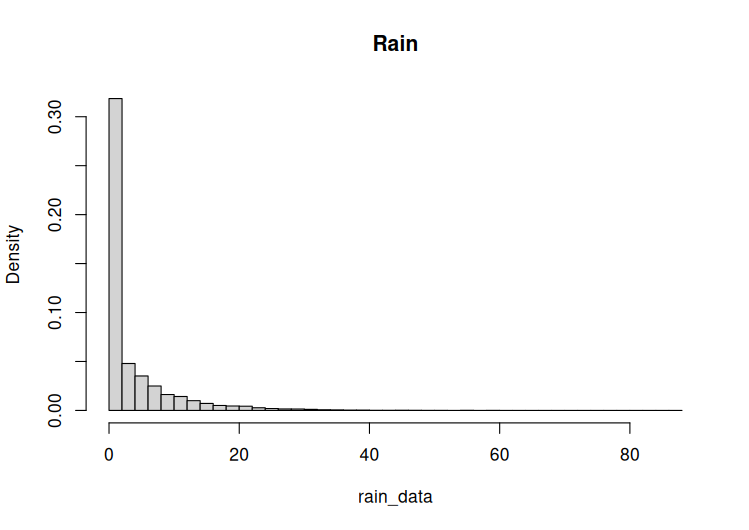
\includegraphics[scale=0.62]{./images/rainhisto.png} 
\end{center}


\noindent Pour les sinistres, on remarque que la majorité des montants sont de faible intensité mais qu'il existe des sinistres avec des valeurs élevé. Les données se répartissent de $1$ à $263.500$ avec une moyenne de $3,385$ et une médiane de $1,778$. Dans le même cas que dans les données de rain, on peut donc s'attendre à une valeur de gamma positive ou nulle.
\begin{center}
	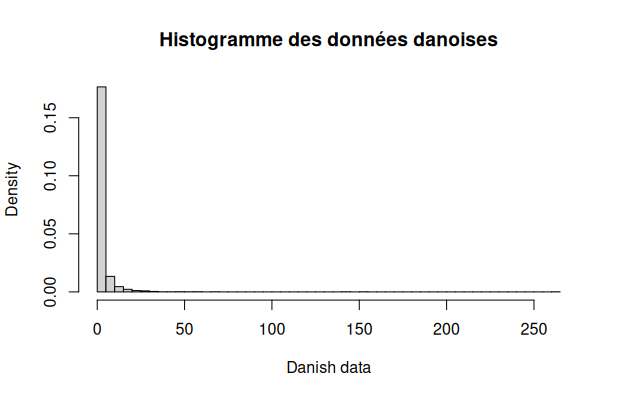
\includegraphics[scale=0.62]{./images/sinistres.png} 
\end{center}

\subsection{Méthode des maxima par bloc}

\subsubsection{Application sur les données de Rain}

\noindent Les données étant journalières, on va choisir des blocs de taille 365, comme les données vont de 1914 à 1962, on se retrouve avec 48 blocs de 365 jours.
\\
Via le package \textbf{evd}, on obtient via une estimations par maximum de vraisemblance les paramètres suivants : $\mu = 40,8$, $\sigma = 9,73$ et $\gamma = 0,107$.
\\
L'estimation des paramètres sont calculées par maximum de vraisemblance.
\\
\\
On suppose alors que $\gamma \geq 0$, donc il n’existe pas de valeur maximale finie : la probabilité de très gros maxima décroît mais n'est pas finie, selon un comportement polynomial ou exponentiel ce qui est embettant dans le cas pratique surtout quand on cherche des seuils rarement atteints.
\\
\\
On calcule alors le quantile de retour pour $T=100$ afin d'avoir une valeur de pluie qui ne devrait pas être dépassée plus d'une fois tous les 100 ans.
\\
\\
On obtient alors : $z_t = 98,636$. Autrement dit, une fois tous les 100 ans, on peut s'attendre à avoir une pluie de plus de 98.636 mm.




\subsubsection{Application sur les données danish}
\noindent On applique la même méthode sur les données de sinistres mais avec une approche légèrement différente puisque les données ne sont pas dans le même format. En effet, on ne dispose pas de données journalières mais des sinistres enregistré sur une période de 10 ans. C'est à dire qu'il existe des jours sans sinistres qui ne sont pas comptabilisés.
On regroupe alors les sinistres par mois et on prend le montant de sinistre le plus élevé. On se retrouve alors avec des blocs de taille irrégulière.
\\
Après analyse numérique par maximum de vraisemblance, on obtient les paramètres suivants : $\mu = 8,376$, $\sigma = 5,971$ et $\gamma = 0,623$.
\\
\\
On peut alors calculer le quantile de retour pour $T=50$ afin d'avoir une valeur de sinistre qui ne devrait pas être dépassée plus d'une fois tous les 50 ans.
\\
\\
On obtient alors : $z_t = 515,22$. Autrement dit, une fois tous les 50 ans, on peut s'attendre à avoir un sinistre depassant plus de $515,22$.

\subsubsection{Synthèse sur la méthode des maxima en bloc}

\noindent Quand on dispose des données sur une longue période, la méthode des maxima en bloc est efficace. D'autant plus quand on a des données temporelles (journalières, mensuelles, annuelles).
En revanche, elle utilise moins de données ce qui la rend plus difficile à utiliser en pratique. En effet, on ne garde que les maximums et on perd donc une partie des données qui peuvent etre consequents en fonction du choix de $k$.
Par ailleurs, le choix de $k$ est important car il faut choisir un nombre de blocs suffisant pour avoir une estimation fiable mais pas trop grand pour ne pas perdre trop d'informations.

\subsection{Méthode de dépassement de seuil}


\subsubsection{Application sur les données de Rain}

\noindent On a calculé la valeur de $\gamma$ par la méthode des maxima en bloc et obtenu une valeur de $\gamma > 0 $ mais proche de 0. On souhaite s'assurer de l'efficacité des deux méthodes $\gamma$
en procédant cette fois par la méthode de dépassement de seuil.
\\
On décide de prendre un seuil correspondant au quantile d’ordre 0,95 et on obtient numériquement : $\gamma  = -0.027$.
\\
\\
On a obtenu dans la méthode des maxima en bloc une valeur de $\gamma$ postive mais proche de 0,
tandis qu'avec la méthode de dépassement de seuil, on obtient une valeur négative mais tout aussi proche de 0.
\\
On peut poursuivre l'étude en calculant la valeur de $\gamma$ via l'estimateur de Pickands.

\begin{center}
	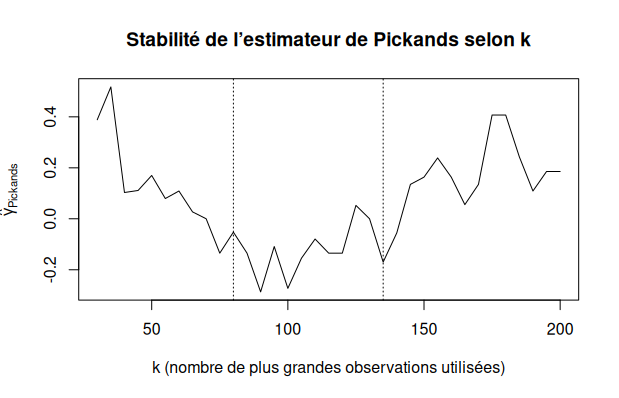
\includegraphics[scale=0.57]{./images/pickandsrain.png} 
\end{center}

\noindent On observe qu'il y'a une stabilisation de l'estimateur de Pickands pour $k$ entre 80 et 135. On obtient alors apres estimation numérique une valeur de $\gamma = -0,079$.
\\
\\
Étant donnée qu'on a obtenu plusieurs valeurs de $\gamma$ positives et négatives, on pourrait procéder à un test de significativité pour savoir si la valeur de $\gamma$ est différente de 0. Nous omettons cette partie et supposons que $\gamma$ est égal à 0. C'est à dire que le maximum de pluie suit une loi de Gumbel.
\\
\subsubsection{Application sur les données danish}

\noindent On prend un seuil correspondant au quantile d’ordre 0,95. Apres calcul numérique, on obtient $\gamma = 0.492$.
\\
On a obtenue une valeur de $\gamma$ positive ce qui renforce l'hypothèse d'une queue lourde pour la distribution du max, ce qui est cohérent avec la méthode des maxima en bloc. 
\\
Avec l'estimateur de Pickands, on observe une stabilisation de l'estimateur pour $k$ entre 70 et 110. On obtient alors apres estimation numérique une valeur de $\gamma = 0.938$. Un résultat assez haut qui est due à l'instabilité de l'estimateur de Pickands. 

\begin{center}
	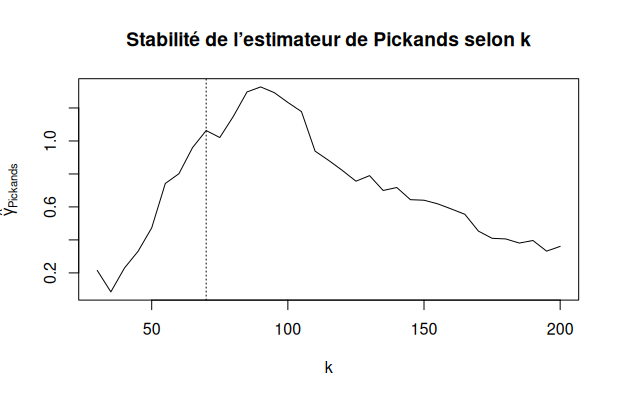
\includegraphics[scale=0.65]{./images/pickandsdansih.png} 
\end{center}




\noindent Ayant plusieurs fois obtenue un valeur de $\gamma > 0$, on peut pousser son analyse en calculant son estimation via l'estimateur de Hill pour obtenir une valeur plus précise.
\\
\\
On trace alors la courbe de l'estimateur de Hill en fonction de $k$.

\begin{center}
	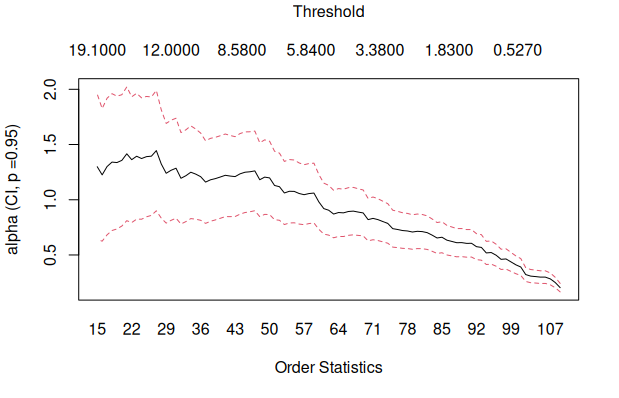
\includegraphics[scale=0.65]{./images/danishsad.png} 
\end{center}

\noindent On observe alors un plateau pour k entre 30 et 45. On obtient alors apres estimation numérique une valeur de $\gamma = 0,66$.

\subsubsection{Synthèse sur la méthode de dépassement de seuil}
\noindent Cette méthode à le bon goût d'exploiter toutes les valeurs supérieures à un seuil, pas seulement un maximum par bloc. Elle utilise donc plus de données.
\\
En revanche le choix du seuil est important car il faut choisir un seuil suffisamment élevé pour ne pas avoir trop peu de données mais pas trop élevé pour ne pas perdre d'informations sur les max. Il faut donc faire le compromis entre le biais et la variance.

\section{Conclusion}

Dans ce projet, nous avons exploré la \textbf{théorie des valeurs extrêmes}, un cadre probabiliste permettant de modéliser les événements rares et extrêmes. 
La démonstration de la convergence des maxima d’échantillons vers une loi de valeurs extrêmes a été au cœur de notre étude. Cette loi dépend de trois paramètres : un paramètre de localisation $\mu$, un paramètre d’échelle $\sigma > 0$, et un paramètre de forme $\gamma$, qui gouverne le comportement de la queue.
\\
Ce paramètre de forme $\gamma$ est le plus important à estimer en pratique. En effet, il permet de connaître le comportement de la queue de la distribution.
L'estimation de ce paramètre à prit une bonne partie de notre projet. Nous avons utilisé
des méthodes \textbf{non paramétriques} : les estimateurs de \textbf{Hill} (adapté aux queues lourdes, $\gamma > 0$) et de \textbf{Pickands}, permettant une estimation robuste de $\gamma$ à partir des ordres statistiques des excès,



\medskip

Nous avons appliqué ces méthodes à plusieurs jeux de données réelles, comme les hauteurs de pluie (\texttt{rain}) ou les sinistres danois (\texttt{danish}). Ces analyses nous ont permis d'estimer les paramètres extrêmes, d'évaluer le risque de valeurs rares et de calculer des \textbf{quantiles de retour} (niveaux censés être dépassés tous les $T$ ans).

\medskip

Nous aurions pu approfondir notre étude en réalisant des tests de significativité pour déterminer le signe de $\gamma$ comme par exemple le test de van Montfort et Otten, mais nous avons choisi de nous concentrer sur l'estimation et l'interprétation des résultats par souci de temps.

\medskip

Ainsi, la théorie des valeurs extrêmes s’avère être un outil indispensable pour la modélisation des événements rares dans de nombreux domaines appliqués (hydrologie, finance, assurance, climatologie, etc.). Une bonne estimation du paramètre de forme $\gamma$ est essentielle pour la prise de décision en conditions extrêmes.


\newpage
\section{Annexe}
\subsection{Quelques simulations pour les méthodes de maxima par blocs et dépassement de seuil}

\noindent Quelques illustrations simulées des méthodes vues dans le texte pour les lois uniforme, normale et de Cauchy. \\
\noindent Les codes des simulations suivantes sont disponibles sur Github dans les sous dossiers Codes Dépassement-Seuil et Codes Maxima-Blocs du dossier CodesR.

\subsubsection{Maxima par blocs}

\begin{center}
	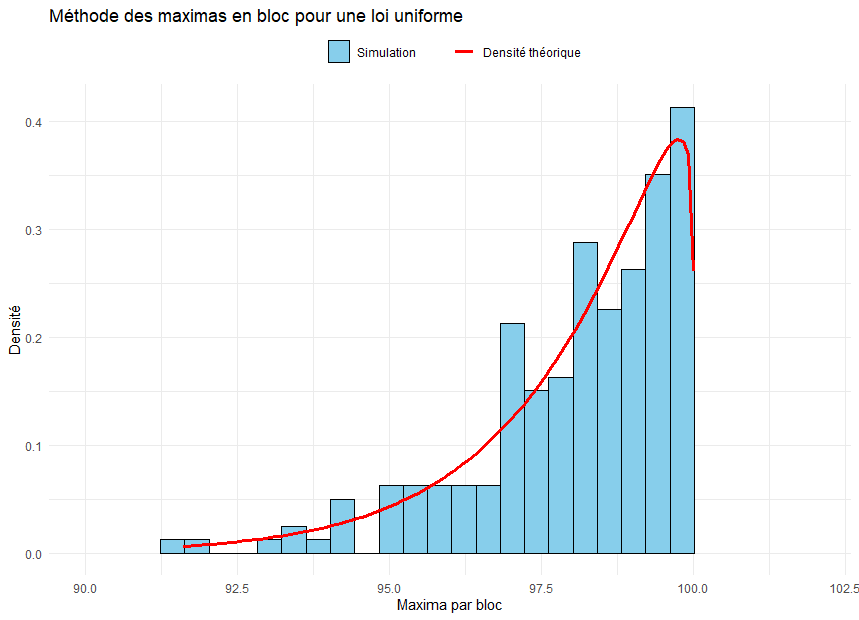
\includegraphics[scale=0.60]{./images/MB_Uniforme} 
\end{center}

\begin{center}
	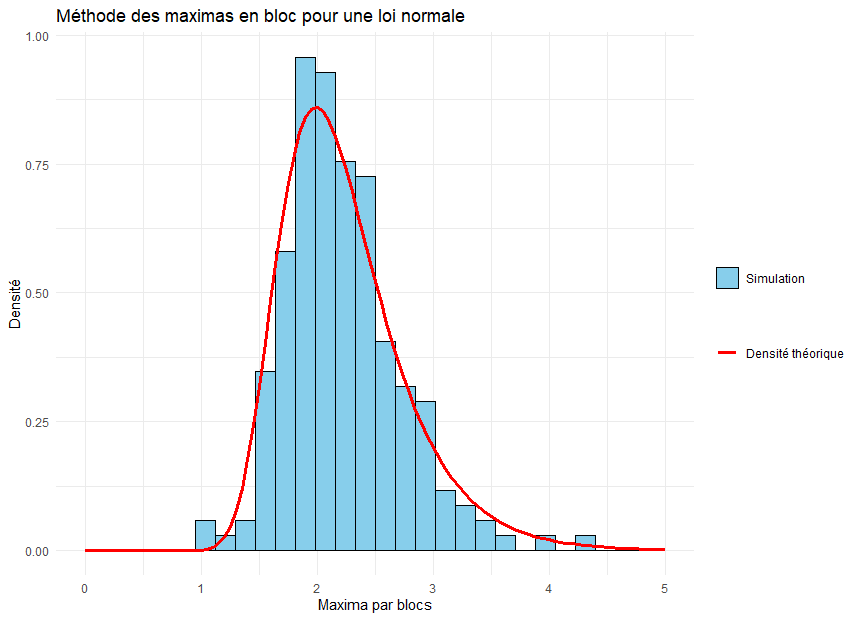
\includegraphics[scale=0.60]{./images/MB_Normale} 
\end{center}

\begin{center}
	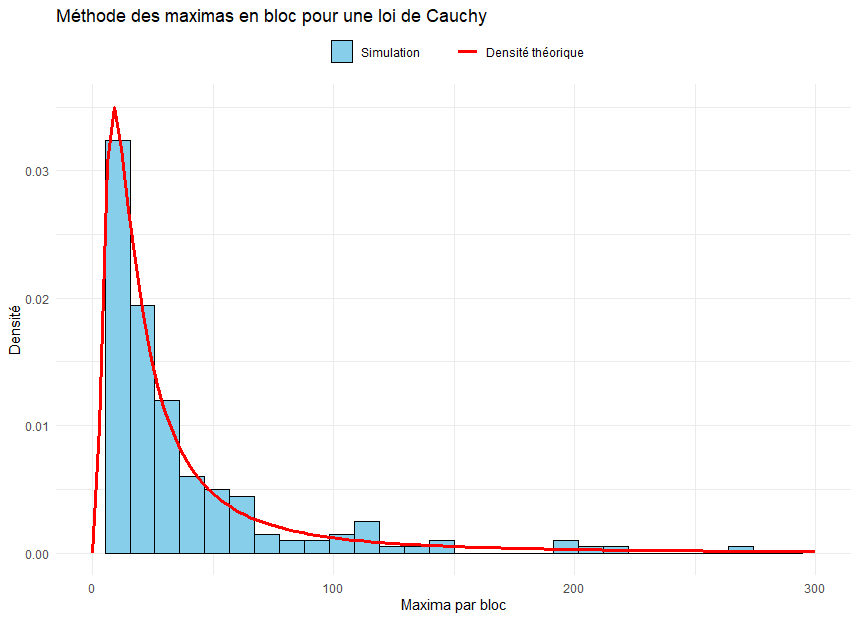
\includegraphics[scale=0.60]{./images/MB_Cauchy} 
\end{center}

\subsubsection{Dépassements de seuil}

\begin{center}
	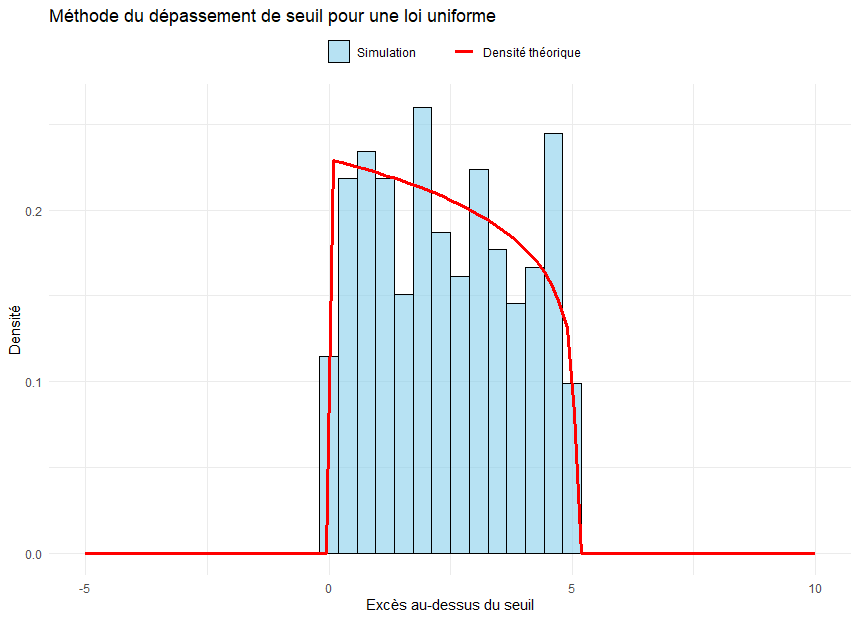
\includegraphics[scale=0.60]{./images/DS_Uniforme} 
\end{center}

\begin{center}
	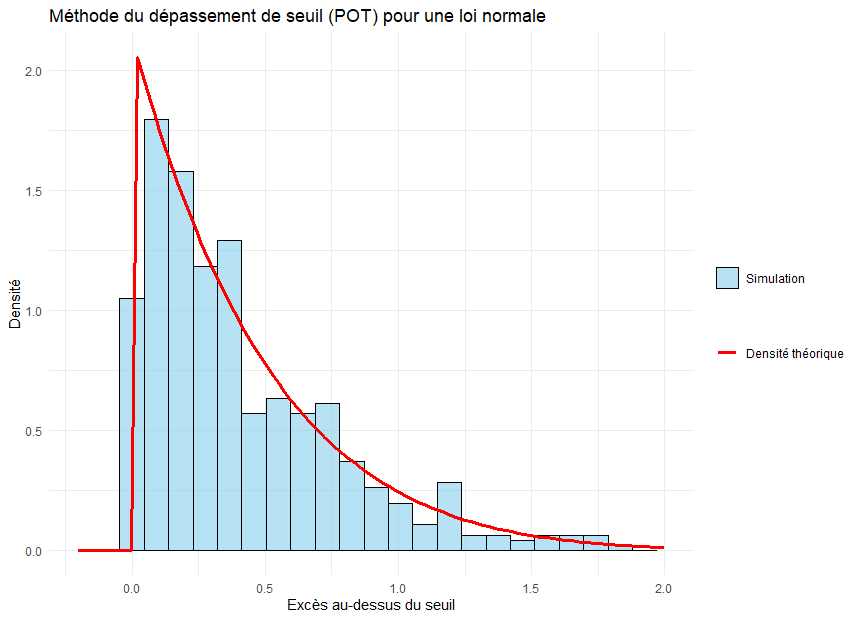
\includegraphics[scale=0.60]{./images/DS_Normale} 
\end{center}

\begin{center}
	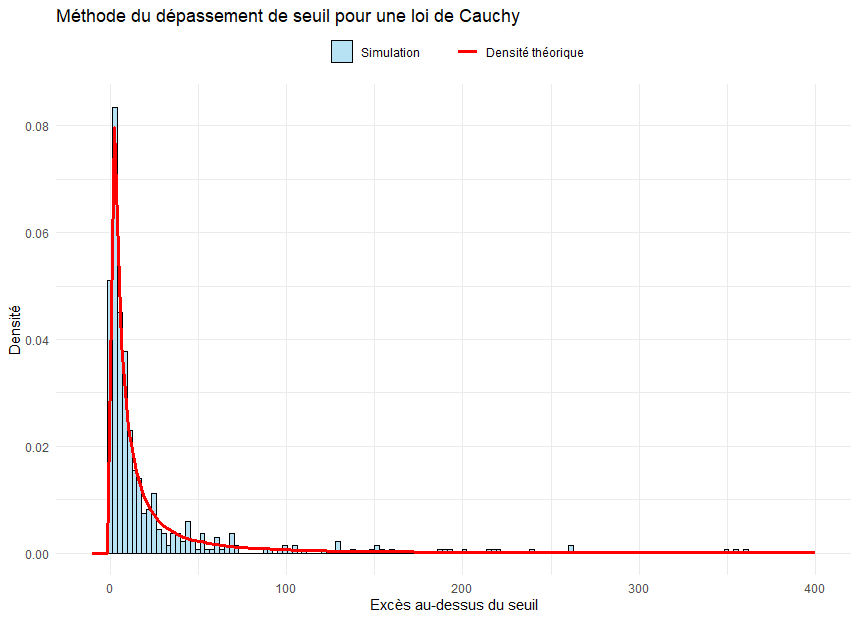
\includegraphics[scale=0.60]{./images/DS_Cauchy} 
\end{center}

\subsection{Codes R}

\noindent Le code pour pour les sorties graphiques et les calculs des estimateurs sont disponible sur le github du projet : https://github.com/DamienMariac/HAX817X-Projet.

\newpage
\section*{Bibliographie}

\begin{itemize}
	\item An Introduction to Statistical Modeling of Extreme Values, Stuart Coles 2001
	\item Modelling Extremal Events  Paul Embrechts , Claudia Klüppelberg , Thomas Mikosch
	\item Statistics of Extremes Theory and Applications, Jan Beirlant, Yuri Goegebeur, Johan Segers, Jozef Teugels
	\item Bibm@th.net
	\item Théorie des valeurs extrêmes et estimation de mesures de risque, Jonathan El Methni, Gilles Stupfler
	\item On The Limiting Distribution of the Maximum Term in a Random Series, Boris Vladimirovitch Gnedenko
	\item Estimation non-paramétrique des quantiles extrêmes conditionnels, Imene Bouazza, Mémoire de Master, Université de Saïda - Dr Moulay Tahar, 2018
	\item Méthodes non paramétriques d’estimation des quantiles extrêmes conditionnels, Jonathan El Methni, Mémoire de Master, École normale supérieure de Cachan, 2015
	\item Yoann, Estimateur de Hill – Illustration avec R, RPubs, 2019. \url{https://rpubs.com/Yoann/499582}
\end{itemize}

\end{document}